\documentclass[12pt,a4paper]{article}
\usepackage{tikz}
\usetikzlibrary{arrows}
\usepackage{latexsym}
\usepackage{tech,mathsx,mytheorems,url}
\usepackage{cspm}
\usepackage{scalalistings}

\newtheorem{lemma}{Lemma}
\newtheorem{definition}[lemma]{Definition}
\newtheorem{prop}[lemma]{Proposition}
\newtheorem{example}[lemma]{Example}

\def\s#1{$_{#1}$}
\def\call{\mathsf{call}}
\def\return{\mathsf{return}}
\def\::{\mathord{\hspace{0.1mm}:\hspace{0.1mm}}}
\def\range#1#2{[#1 \mathbin{..} #2)}
\def\op{{\sm{op}}}
\def\sync{\sm{sync}}
\def\send{\sm{send}}
\def\receive{\sm{receive}}

% tikz stuff

\def\X{node {$\cross$}}
% Bullet at (#1,#2) with text #3 below
\def\bulletAt(#1,#2)#3{%
  \draw(#1,#2) node {$\bullet$}; \draw(#1,#2-0.4) node{\footnotesize #3};
}
% Cross at (#1,#2) with text #3 below
\def\crossAt(#1,#2)#3{%
  \draw(#1,#2) \X; \draw(#1,#2-0.4) node{\footnotesize #3};
}

\def\topfraction{0.75}
\renewcommand{\floatpagefraction}{0.7}

\sloppy\raggedbottom

\title{Understanding Synchronisation}
\author{Jonathan Lawrence and Gavin Lowe}

\begin{document}
\maketitle

\begin{abstract}
\ldots
\end{abstract}

%%%%%%%%%%%%%%%%%%%%%%%%%%%%%%%%%%%%%%%%%%%%%%%%%%%%%%%


\section{Introduction}

A common step of many concurrent programs involves two or more threads
\emph{synchronising}: each thread waits until other relevant threads have
reached the synchronisation point before continuing; in addition, the threads
can exchange data.  Reasoning about programs can be easier when
synchronisations are used: it helps us to reason about the states that
different threads are in. 

We study synchronisations in this paper: we formalise the requirements of
synchronisations, and describe testing and analysis techniques.

We start by giving some examples of synchronisations in order to illustrate
the idea.  (We use Scala notation; we explain non-standard aspects of the
language in footnotes.)  In each case, the synchronisation is mediated by a
\emph{synchronisation object}.

Perhaps the most common form of synchronisation object is a synchronous
channel.  Such a channel might have signature\footnote{The type {\scalashape
    Unit} is the type that contains a single value, the \emph{unit value},
  denoted~{\scalashape ()}.}
%
\begin{scala}
class SyncChan{
  def send(x: A): Unit
  def receive(): A
}
\end{scala}
%
Each invocation of one of the operations must synchronise with an invocation
of the other operation: the two invocations must overlap in time.  If an
invocation |send(x)| synchronises with an invocation of |receive|, then the
|receive| returns~|x|.

Sometimes an invocation may synchronise with an invocation of the same
operation.  For example, an \emph{exchanger} has the following signature.
%
\begin{scala}
class Exchanger{
  def exchange(x: A): A
}
\end{scala}
%
When two threads call |exchange|, they each receive the value passed in by the
other.  When invocations of two different operations synchronise, we use the
term \emph{heterogeneous}; where two invocations of the same operation
synchronise, we use the term \emph{homogeneous}.  

For some synchronisation objects, synchronisations might involve more than two
threads.  For example, an object of the following class
%
\begin{scala}
class Barrier(n: Int){
  def sync(): Unit
}
\end{scala}
%
can be used to synchronise~|n| threads, known as a \emph{barrier
  synchronisation}: each thread calls |sync|, and no invocation returns until
all~|n| have called it.

A \emph{combining barrier} also allows each thread to submit a parameter, and
for all to receive back some function of those parameters.\footnote{The Scala
  type {\scalastyle (A,A) =}$>$ {\scalastyle A} represents functions from
  pairs of {\scalastyle A} to~{\scalastyle A}.}
%
\begin{scala}
class CombiningBarrier(n: Int, f: (A,A) => A){
  def sync(x: A): A
}
\end{scala}
%
The function |f| is assumed to be associative.  If |n| threads call |sync|
with parameters $x_1, \ldots, x_{\ss n}$, in some order, then each receives
back $\sm f(x_1, \sm f(x_2, \ldots \sm f(x_{{\ss n}-1}, x_{\ss n}) \ldots ))$
(in the common case that |f| is commutative, this result is independent of the
order of the parameters).

In addition, we allow the synchronisations to be mediated by an object that
maintains some state between synchronisations.  As an example, consider a
synchronous channel that, in addition, maintains a sequence counter, and such
that both invocations receive the value of this counter.
\begin{scala}
class SyncChanCounter{
  private var counter: Int
  def send(x: A): Int
  def receive(): (A, Int)
}
\end{scala}

% Variations: homogenous case; different modes


Some synchronisation objects allow different modes of synchronisation.  For
example, consider a synchronous channel with timeouts: each invocation might
synchronise with another invocation, or might timeout without
synchronisation.  Such a channel might have a signature as follows.
%
\begin{scala}
class TimeoutChannel{
  def send(x: A): Boolean
  def receive(): Option[A]
}
\end{scala}
%
The |send| operation returns a boolean to indicate whether the send was
successful, i.e.~whether it synchronised.  The |receive| operation can return
a value |Some(x)| to indicate that it synchronised and received~|x|, or can
return the value |None| to indicate that it failed to synchronise\footnote{The
  type {\scalashape Option[A]} contains the union of such values.}.  Thus an
invocation of each operation may or may not synchronise with an invocation of
the other operation. 

A \emph{termination-detecting queue} can also be thought of as a stateful
synchronisation object with multiple modes.  Such an object acts like a
standard partial concurrent queue: if a thread attempts to dequeue, but the
queue is empty, it blocks until the queue becomes non-empty.  However, if a
state is reached where all the threads are blocked in this way, then they all
return a special value to indicate this fact.  In many concurrent algorithms,
such as a concurrent graph search, this latter outcome indicates that the
algorithm should terminate.  Such a termination-detecting queue might have the
following signature, where a dequeue returns the value |None| to indicate the
termination case.
%
\begin{scala}
class TerminationDetectingQueue(n: Int){ // £n£ is the number of threads   
  def enqueue(x: A): Unit
  def dequeue: Option[A]
}
\end{scala} 
%
The termination outcome can be seen as a synchronisation between all |n|
threads.  This termination-detecting queue combines the functionality of a
concurrent datatype and a synchronisation object.


%% In general, a synchronisation will involve some number~$k$ of threads, calling
%% operations of the form
%% %
%% \begin{scala}
%%   def op£\s1£(x£\s1£: A£\s1£): B£\s1£
%%   ...
%%   def op£\s k£(x£\s k£: A£\s k£): B£\s k£
%% \end{scala}
%% %
%% Each thread passes in some data, and receives back a result. 

In this paper, we consider what it means for one of these synchronisation
objects to be correct, and techniques for testing correctness.  

In Section~\ref{sec:spec} we describe how to specify a synchronisation
object.  The definition has similarities with the standard definition of
\emph{linearisation} for concurrent datatypes, except it talks about
synchronisations between invocations, rather than single invocations: we call
the property \emph{synchronisation linearisation}. 

In Section~\ref{sec:relating} we consider the relationship between
synchronisation linearisation and (standard) linearisation.  We show that the
two notions are different; but we show that synchronisation linearisation
corresponds to a small adaptation of linearisation, where an
operation of the synchronisation object may correspond to \emph{two} operations
of the object used to specify linearisation.  

We then consider testing of synchronisation object implementations.  Our
techniques are based on the techniques for testing (standard)
linearisation~\cite{gavin:lin-testing}, which we sketch in
Section~\ref{sec:lin-testing}.  In Section~\ref{sec:testing-hacking} we show
how the technique can be adapted to test for synchronisation linearisation,
using the result of Section~\ref{sec:relating}.  Then in
Section~\ref{sec:direct} we show how synchronisation linearisation can be
tested more directly, and present various complexity results.

In Section~\ref{sec:modelChecking} we consider how the property of
synchronisation linearisation can be analysed via model checking.  


\section{Specifying synchronisations}
\label{sec:spec}

In this section we describe how synchronisations can be formally specified.
For ease of exposition, we start by \emph{heterogeneous binary}
synchronisation in this section, where every synchronisation is between
invocations of two different operations.
We generalise at the end of this section.

We assume that the synchronisation object has two operations, each of which
has a single parameter, with signatures as follows.
%
\begin{scala}
  def op£\s1£(x£\s1£: A£\s1£): B£\s1£
  def op£\s2£(x£\s2£: A£\s2£): B£\s2£
\end{scala}
%
(We can model a concrete operation that takes $k > 1$ parameters by an
operation that takes a $k$-tuple as its parameter; we can model a concrete
operation that takes no parameters by an operation that takes a |Unit|
parameter.) 
%
In addition, the synchronisation object might have some state, |state: S|.
Each invocation of~|op|\s1 must synchronise with an invocation of~|op|\s2, and
vice versa.  The result of each invocation may depend on the two parameters
|x|$_1$ and |x|$_2$ and the current state.  In addition, the state may be
updated.  The external behaviour is consistent with the synchronisation
happening atomically at some point within the duration of both operation
invocations (which implies that the invocation must overlap): we refer to this
point as the \emph{synchronisation point}.

Each synchronisation object can be specified using a \emph{synchronisation
  specification object} with the following signature.
%
\begin{scala}
class Spec{
  def sync(x£\s1£: A£\s1£, x£\s2£: A£\s2£): (B£\s1£, B£\s2£)
}
\end{scala}
%
The idea is that if two invocations |op|\s1|(x|\s1|)| and |op|\s2|(x|\s2|)|
synchronise, then the results |y|\s1 and |y|\s2 of the invocations are such
that $\sm{sync}(\sm x_1, \sm x_2)$ could return the pair |(y|\s1|, y|\s2|)|.
The specification object might have some private state that is accessed and
updated within~|sync|.  Note that invocations of |sync| occur
\emph{sequentially}.

We formalise below what it means for a synchronisation object to satisfy the
requirements of a synchronisation specification object.  But first, we give
some examples to illustrate the style of specification. 

A typical definition of the specification obejct might take the following form
%
\begin{scala}
class Spec{
  private var state: S
  def sync(x£\s1£: A£\s1£, x£\s2£: A£\s2£): (B£\s1£, B£\s2£) = {
    require(guard(x£\s1£, x£\s2£, state))
    val res£\s1£ = f£\s1£(x£\s1£, x£\s2£, state); val res£\s2£ = f£\s2£(x£\s1£, x£\s2£, state)
    state = update(x£\s1£, x£\s2£, state)
    (res£\s1£, res£\s2£)
  }
}
\end{scala}
%
The object has some local state, which persists between invocations.  The
|require| clause of |sync| specifies a precondition for the synchronisation to
take place.  The values |res|\s1 and |res|\s2 represent the results that
should be returned by the corresponding invocations of~|op|\s1 and~|op|\s2,
respectively.  The function |update| describes how the local state should be
updated. 

For example, consider a synchronous channel with operations
\begin{scala}
  def send(x: A): Unit
  def receive(u: Unit): A
\end{scala}
%
(Note that we model the |receive| operation as taking a parameter of type
|Unit|, in order to fit our uniform setting.) 
%
This can be specified using a synchronisation specification object as follows,
with empty state
\begin{scala}
class SyncChanSpec{
  def sync(x: A, u: Unit): (Unit, A) = ((), x)
}
\end{scala}
%
If |send(x)| synchronises with |receive(())|, then the former receives the
unit value~|()|, and the latter receives~|x|. 

As another example, consider a filtering channel.
\begin{scala}
class FilterChan{
  def send(x: A): Unit
  def receive(p: A => Boolean): A
}
\end{scala}
%
Here the |receive| operation is passed a predicate~|p| describing a required
property of any value received.  This can be specified using a specification
object with operation
%
\begin{scala}
  def sync(x: A, p: A => Boolean): (Unit, A) = { require(p(x)); ((), x) }
\end{scala}
%
Invocations |send(x)| and |receive(p)| can synchronise only if |p(x)|. 

As an example illustrating the use of state in the synchronisation object,
recall the synchronous channel with a sequence counter, |SyncChanCounter|,
from the introduction.  This can be specified using the following
specification object.
%
\begin{scala}
class SyncChanCounterSpec{
  private var counter = 0
  def sync(x: A, u: Unit): (Int, (A, Int)) = {
    counter += 1; (counter, (x, counter))
  }
}
\end{scala}

%%%%%%%%%%

\subsection{Linearisability}
\label{sec:specification-linearisability}

We formalise below precisely the allowable behaviours captured by a particular
synchronisation specification object.  Our definition has much in common with
the well known notion of \emph{linearisation}~\cite{herlihy-wing}, used for
specifying concurrent datatypes; so we start by reviewing that notion.  There
are a number of equivalent ways of defining linearisation: we choose a way
that will be convenient subsequently.

A \emph{concurrent history} of an object~$o$ (either a concurrent datatype or
a synchronisation object) records the calls and returns of operation
invocations on~$o$.  It is a sequence of events of the following forms:
%
\begin{itemize}
\item $\call.op^i(x)$, representing a call of operation~$op$ with
  parameter~$x$;
\item $\return.op^i \:: y$, representing a return of an invocation of~$op$,
  giving result~$y$.
\end{itemize}
%
In each case, $op$ is an operation of~$o$.  Here $i$ is a \emph{invocation
  identity}, used to identify a particular invocation, and to link the $\call$
and corresponding~$\return$.  In order to be well formed, each invocation
identity must appear on at most one $\call$ event and at most one $\return$
event; and for each event $\return.op^i\::y$, the history must contain an
earlier event $\call.op^i(x)$, i.e.~for the same operation and invocation
identity.  We consider only well formed histories from now on.  We say that a
$\call$ event and a $\return$ event \emph{match} if they have the same
invocation identifier.  A concurrent history is \emph{complete} if for every
$\call$ event, there is a matching $\return$ event, i.e.~no invocation is
still pending at the end of the history.

For example, consider the following complete concurrent history of a
concurrent object that is intended to implement a queue, with operations |enq|
and~|deq|.
%
\begin{eqnarray*}
h & = & 
  \seq{\begin{align}
    \call.\sm{enq}^1(5),\; \call.\sm{enq}^2(4),\; \call.\sm{deq}^3(), \\
    \return.\sm{enq}^1\::(),\; \return.\sm{deq}^3\::4,\;
    \return.\sm{enq}^2\::() }.
    \end{align}
\end{eqnarray*}
%
This history is illustrated by the timeline in Figure~\ref{fig:lin-timeline}:
here, time runs from left to right; each horizontal line represents an
operation invocation, with the left-hand end representing the $\call$ event,
and the right-hand end representing the $\return$ event. 

%%%%%

\begin{figure}
\unScalaMid
\def\X{node{$\cross$}}
\begin{center}
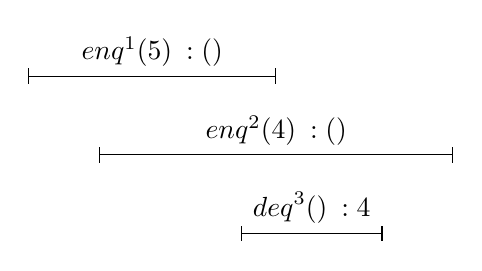
\begin{tikzpicture}[xscale = 0.9]
\draw[|-|] (0,0) -- node[above] {$\sm{enq}^1(5)\::()$} (3.5,0);
\draw (2.5,0) \X;
\draw[|-|] (1,-1) -- node[above] {$\sm{enq}^2(4)\::()$} (6,-1);
\draw (2,-1) \X;
\draw[|-|] (3,-2) -- node[above] {$\sm{deq}^3()\::4$} (5,-2);
\draw (4,-2) \X;
\end{tikzpicture}
\end{center}
\caption{Timeline representing the linearisation example.}
\label{fig:lin-timeline}
\scalaMid
\end{figure}

%%%%%

Linearisability is specified with respect to a specification object~$Spec$,
with the same operations (and signatures) as the concurrent object in
question.  A history of the specification object is a sequence of events of
the form:
%
\begin{itemize}
\item $op^i(x):y$ representing an invocation of operation~$op$ with
  parameter~$x$, returning result~$y$; again $i$~is an invocation identity,
  which must appear at most once in the history.
\end{itemize}
%
A history is \emph{legal} if it is consistent with the definition of~$Spec$,
i.e.~for each invocation, the precondition is satisfied, and the return value
is as for the definition of the operation in~$Spec$.

For example, consider the history
\begin{eqnarray*}
h_s & = & \seq{\sm{enq}^2(4)\::(),\; \sm{enq}^1(5)\::(),\; \sm{deq}^3\::4}.
\end{eqnarray*}
%
This is a legal history for a specification object that represents a queue.
This history is illustrated by the ``$\cross$''s in
Figure~\ref{fig:lin-timeline}.

Let $h$ be a complete concurrent history, and let $h_s$ be a legal history of
the specification object corresponding to the same invocations, i.e., for each
$\call.op^i(x)$ and $\return.op^i\::y$ in $h$,\, $h_s$ contains $op^i(x)\::y$,
and vice versa.  We say that $h$ and~$h_s$ are \emph{compatible} if there is
some way of interleaving the two histories (i.e.~creating a history containing
the events of~$h$ and~$h_s$, preserving the order of events) such that each
$op^i(x)\::y$ occurs between $\call.op^i(x)$ and $\return.op^i\::y$.
Informally, this indicates that the invocations of~$h$ appeared to take place
in the order described by~$h_s$, and that that order is consistent (in terms
of the satisfaction of preconditions and values returned) with the
specification object.

Continuing the running example, the histories $h$ and~$h_s$ are compatible, as
evidenced by the interleaving
\[
\seq{\begin{align}
  \call.\sm{enq}^1(5),\; \call.\sm{enq}^2(4),\; 
  \sm{enq}^2(4)\::(),\; \sm{enq}^1(5)\::(),\;   \call.\sm{deq}^3(), \\
  \return.\sm{enq}^1\::(),\; \sm{deq}^3\::4,\; 
  \return.\sm{deq}^3\::4,\; \return.\sm{enq}^2\::() },
  \end{align}
\]
which is again illustrated in  Figure~\ref{fig:lin-timeline}.

We say that a complete history~$h$ is \emph{linearisable} with respect to
$Spec$ if there is a corresponding valid history~$h_s$ of~$Spec$ such that $h$
and~$h_s$ are compatible.  

A concurrent history might not be complete, i.e.~it might have some pending
invocations.  An \emph{extension} of a history~$h$ is formed by adding zero or
more $\return$ events corresponding to pending invocations.  We write
$complete(h)$ for the subsequence of~$h$ formed by removing all $\call$ events
corresponding to pending invocations. 
%
We say that a (not necessarily complete) concurrent history~$h$ is
\emph{linearisable} if there is an extension~$h'$ of~$h$ such that
$complete(h')$ is linearisable.  We say that a concurrent object is
linearisable if all of its histories are linearisable. 

%%%%%

\subsection{Synchronisation linearisability}

We now adapt the definition of linearisability to synchronisations.  We
consider a concurrent history of the synchronisation object~$Sync$, as with
linearisability; in the case of binary synchronisation, this will contain
events corresponding to the operations~$op_1$ and~$op_2$.

For example, the following is a complete history of the synchronous channel
from earlier, and is illustrated in Figure~\ref{fig:sync-timeline}:
\begin{eqnarray*}
h & = & 
\seq{\begin{align}
  \call.\sm{send}^1(8),\; \call.\sm{send}^2(8),\; \call.\sm{receive}^3(()),\;
  \return.\sm{receive}^3\::(),\; \\
  \call.\sm{receive}^4(()),\; \return.\sm{send}^1\::(),\;
  \call.\sm{send}^5(9),\; \return.\sm{receive}^4\::9,\; \\
  \call.\sm{receive}^6(()),\; \return.\sm{send}^2\::(), \;
  \return.\sm{send}^5\::(),\; \return.\sm{receive}^6\::8 } .
  \end{align}
\end{eqnarray*}

%%%%%

\begin{figure}
\unScalaMid
\def\X{node {$\cross$}}
\begin{center}
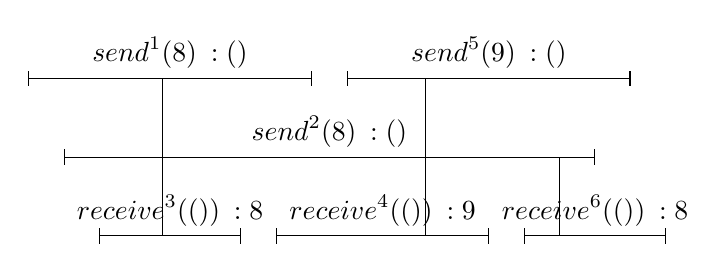
\begin{tikzpicture}[xscale = 0.9]
\draw[|-|] (0,0) -- node[above] {$\sm{send}^1(8)\::()$} (4,0);
\draw[|-|] (4.5,0) -- node[above] {$\sm{send}^5(9)\::()$} (8.5,0);
\draw[|-|] (0.5,-1) -- node[above] {$\sm{send}^2(8)\::()$} (8,-1);
\draw[|-|] (1,-2) -- node[above] {$\sm{receive}^3(())\::8$} (3,-2);
\draw[|-|] (3.5,-2) -- node[above] {$\sm{receive}^4(())\::9$} (6.5,-2);
\draw[|-|] (7,-2) -- node[above] {$\sm{receive}^6(())\::8$} (9,-2);
\draw (1.9,0) \X; \draw (1.9,-2) \X; \draw (1.9,0) -- (1.9,-2); % sync 1 and 3
\draw (5.6,0) \X; \draw (5.6,-2) \X; \draw (5.6,0) -- (5.6,-2); % sync 4 and 5
\draw (7.5,-1) \X; \draw (7.5,-2) \X; \draw (7.5,-1) -- (7.5,-2); % sync 2 and 6 
\end{tikzpicture}
\end{center}
\caption{Timeline representing the synchronisation example.}
\label{fig:sync-timeline}
\scalaMid
\end{figure}


A history of a synchronisation specification object $Spec$ is a sequence of
events of the form
%% \begin{itemize}
%% \item 
$\sm{sync}^{i_1, i_2}(x_1, x_2): (y_1, y_2)$, representing an invocation
  of |sync| with parameters $(x_1, x_2)$ and result $(y_1,y_2)$.  The event's
  invocation identity is~$(i_1,i_2)$: each of~$i_1$ and~$i_2$ must appear at
  most once in the history.
%\end{itemize}

Such a history is \emph{legal} if is consistent with~$Spec$.  Informally, a
|sync| event with identity~$(i_1,i_2)$ represents a synchronisation between
the invocations $op_1^{i_1}$ and $op_2^{i_2}$ in a history of the
corresponding synchronisation object.

For example, the following is a legal history of |SyncChanSpec|.
\begin{eqnarray*}
h_s & = & 
\seq{
 \sm{sync}^{1,3}(8,()) \:: ((), 8), \;
 \sm{sync}^{5,4}(9,()) \:: ((), 9), \;
 \sm{sync}^{2,6}(8,()) \:: ((), 8) } .
\end{eqnarray*}
The history is illustrated by the ``$\cross$''s in
Figure~\ref{fig:sync-timeline}: each event corresponds to the synchronisation
of two operations, so is depicted by two ``$\cross$''s on the corresponding
operations, linked by a vertical line.  This particular synchronisation
specification object is stateless, so in fact any permutation of this history
would also be legal (but not all such permutations will be compatible with the
history of the synchronisation object); but the same will not be true in
general of a specification object with state.

Let $h$ be a complete history of the synchronisation object~$Sync$.  We say
that a legal history~$h_s$ of~$Spec$ \emph{corresponds} to~$h$ if:
%
\begin{itemize}
\item For each |sync| event with identity~$(i_1,i_2)$ in~$h_s$,\, $h$ contains
  an invocation of~$op_1$ with identity~$i_1$ and an invocation of~$op_2$ with
  identity~$i_2$;

\item For each invocation of~$op_1$ with identity~$i_1$ in~$h$,\, $h_s$
  contains a |sync| event with identity~$(i_1,i_2)$ for some~$i_2$;

\item For each invocation of~$op_2$ with identity~$i_2$ in~$h$,\, $h_s$
  contains a |sync| event with identity~$(i_1,i_2)$ for some~$i_1$.
\end{itemize}
%
%% Informally, a |sync| event with identity~$(i_1,i_2)$ represents that the
%% invocations $op_1^{i_1}$ and $op_2^{i_2}$ synchronise.

We say that a complete history $h$ of~$Sync$ and a corresponding legal history
$h_s$ of~$Spec$ are \emph{synchronisation compatible} if there is some way of
interleaving them such that each event $\sm{sync}^{i_1, i_2}(x_1, x_2): (y_1,
y_2)$ occurs between $\call.op_1^{i_1}(x_1)$ and $\return.op_1^{i_1}:y_1$, and
between $\call.op_2^{i_2}(x_2)$ and $\return.op_2^{i_2}:y_2$.

In the running example, the histories~$h$ and~$h_s$ are synchronisation
compatible, as evidenced by the interleaving illustrated in
Figure~\ref{fig:sync-timeline}.

We say that a complete history $h$ of~$Sync$ is \emph{synchronisation
  linearisable} if there is a corresponding legal history $h_s$ of~$Spec$ such
that $h$ and~$h_s$ are synchronisation compatible.

We say that a (not necessarily complete) concurrent history~$h$ is
\emph{synchronisation linearisable} if there is an extension~$h'$ of~$h$ such
that $complete(h)$ is synchronisation linearisable.  We say that a
synchronisation object is synchronisation linearisable if all of its histories
are synchronisation linearisable.

%% Following definition of linearisation.  History of synchronisation object,
%% containing call and return events, with matching invocation indices,
%% e.g. $call.\sm{op}_1^{i_1}(x_1)$ and $return.\sm{op}_1^{i_1}: y_1$; indiced
%% otherwise distinct.  History of sequential specification object, with events
%% representing (atomic) invocations of sync, labelled with a pair of invocation
%% indices, e.g.~$\sm{sync}^{i_1, i_2}(x_1, x_2): (y_1, y_2)$.  No invocation
%% index is repeated in the history.  Define ``legal'' in the normal way.  Define
%% interleaving of concurrent and sequential history: each |sync| has to be
%% between the corresponding $call$ and $return$ for each of the two invocations.

%% Maybe call this \emph{synchronisation linearisation}. 

\framebox{Is the definition compositional?}  I think so.

%%%%%%%%%%%%%%%%%%%%%%%%%%%%%%%%%%%%%%%%%%%%%%%%%%%%%%%

\subsection{Variations}
\label{ssec:spec-variations}

Above we considered heterogeneous binary synchronisations, i.e.~two
invocations of different operations, with a single mode of synchronisation.

It is straightforward to generalise to synchronisations between an arbitrary
number of invocations, some of which might be invocations of the same
operation.  Consider a $k$-way synchronisation between operations
\begin{scala}
  def op£\s j£(x£\s j£: A£\s j£): B£\s j£   £for $j = 1, \ldots, k,$£
\end{scala}
%
where the $op_j$ might not be distinct.
The specification object will have a corresponding operation
%
\begin{scala} 
  def sync(x£\s1£: A£\s1£, ..., x£\s k£: A£\s k£): (B£\s1£, ..., B£\s k£)
\end{scala}
%
For example, for the combining barrier |CombiningBarrier(n, f)| of the
Introduction, the corresponding specification object would be
\begin{scala}
class CombiningBarrierSpec{
  def sync(x£\s1£: A, ..., x£\s n£: A) = {
    val result = f(x£\s1£, f(x£\s2£, ...f(x£\s{{\ss n}-1}£, x£\s{\ss n}£)...)); (result,...,result)
  }
}
\end{scala}

A history of the specification object will have corresponding events
$\sm{sync}^{i_1, \ldots, i_k}(x_1, \ldots, x_k): (y_1, \ldots, y_k)$.
%
The definition of synchronisation compatibility is an obvious adaptation of
earlier: in the interleaving of the complete history of the synchronisation
history and the history of the specification object, each $\sm{sync}^{i_1,
  \ldots, i_k}(x_1, \ldots, x_k): (y_1, \ldots, y_k)$ occurs between
$\call.op_1^{i_j}(x_j)$ and $\return.op_j^{i_j}:y_j$ for each $j = 1, \ldots,
k$.  The definition of synchronisation linearisability follows in the obvious
way. 

It is also straightforward to adapt the definitions to deal with multiple
modes of synchronisation: the specification object has a different operation
for each mode.  For example, recall the |TimeoutChannel| from the
Introduction, where sends and receives may timeout and return without
synchronisation.  The corresponding specification object would be:
%
\begin{scala}
class TimeoutChannelSpec{
  def sync£\s s£(x: A) = false
  def sync£\s r£(u: Unit) = None
  def sync£\s{s,r}£(x: A, u: Unit) = (true, Some(x))
}
\end{scala}
%
The operation $\sm{sync}_s$ corresponds to a send returning without
synchronising; likewise $\sm{sync}_r$ corresponds to a receive returning
without synchronising; and $\sm{sync}_{s,r}$ corresponds to a send and receive
synchronising.  The formal definition of synchronisation linearisation is the
obvious adaptation of the earlier definition.
 % formal definition of synchronisation linearisation
\subsection{Variations}
\label{ssec:spec-variations}

Above we considered heterogeneous binary synchronisations,
i.e.~synchronisations between \emph{two} executions of \emph{different}
operations, with a single mode of synchronisation.

It is straightforward to generalise to synchronisations between an arbitrary
number of operation executions, some of which might be executions of the same
operation.  Consider a $k$-way synchronisation between operations
\begin{scala}
def op£\s j£(x£\s j£: A£\s j£): B£\s j£   £for $j = 1, \ldots, k,$£
\end{scala}
%
where the $\op_j$ might not be distinct.
The specification object will have a corresponding operation
%
\begin{scala} 
def sync(x£\s1£: A£\s1£, ..., x£\s k£: A£\s k£): (B£\s1£, ..., B£\s k£)
\end{scala}
%
For example, for the combining barrier |CombiningBarrier(n, f)| of the
Introduction, the corresponding specification object would be
\begin{scala}
class CombiningBarrierSpec{
  def sync(x£\s1£: A, ..., x£\s{\ss n}£: A) = {
    val result = f(x£\s1£, f(x£\s2£,...f(x£\s{{\ss{n}}-1}£, x£\s{\ss n}£)...)); (result,...,result)
  }
}
\end{scala}

A history of the specification object will have corresponding events
$\sm{sync}^{i_1, \ldots, i_k}(x_1, \ldots, x_k)\:: (y_1, \ldots, y_k)$.
%
The definition of synchronisation linearisation is an obvious adaptation of
earlier: in the interleaving of the complete history of the synchronisation
history and the history of the specification object, each $\sm{sync}^{i_1,
  \ldots, i_k}(x_1, \ldots, x_k)\:: (y_1, \ldots, y_k)$ occurs between
$\call.\op_1^{i_j}(x_j)$ and $\return.\op_j^{i_j}\::y_j$ for each $j = 1,
\ldots, k$.  
%% The definition of synchronisation-linearisability follows in the obvious
%% way.

Note that if several of the $\op_j$ are the same operation, there is a choice
as to the order in which their parameters are passed to |sync|.  (However, in
the case of the combining barrier, if |f| is associative and commutative, the
order makes no difference.)

It is also straightforward to adapt the definitions to deal with multiple
modes of synchronisation: the specification object has a different operation
for each mode.  For example, recall the |TimeoutChannel| from the
Introduction, where sends and receives may timeout and return without
synchronisation.  The corresponding specification object would be:
%
\begin{scala}
class TimeoutChannelSpec[A]{
  def sync£\s s£(x: A) = false       // send times out
  def sync£\s r£(u: Unit) = None  // receive times out
  def sync£\s{s,r}£(x: A, u: Unit) = (true, Some(x))  // synchronisation
}
\end{scala}
%
The operation $\sm{sync}_s$ corresponds to a send returning without
synchronising; likewise $\sm{sync}_r$ corresponds to a receive returning
without synchronising; and $\sm{sync}_{s,r}$ corresponds to a send and receive
synchronising.  The formal definition of synchronisation linearisation is the
obvious adaptation of the earlier definition: in particular |sync|\s{s} must
occur between the call and return of a send that doesn't synchronise, and
likewise for |sync|\s{r}.

As another example, the following is a specification object for a channel with
a close operation.
%
\begin{scala}
class ClosableChannelSpec[A]{
  private var isClosed = false  // is the channel closed? 
  def close(u: Unit) = { isClosed = true; () }
  def sync(x: A, u: Unit) = { require(!isClosed); ((), x)
  def sendFail(x: A) = { require(isClosed); throw new Closed }
  def receiveFail(u: Unit) = { require(isClosed); throw new Closed }
}
\end{scala}
%
A send and receive can synchronise corresponding to |sync|, but only before
the channel is closed; or each may fail once the channel is closed,
corresponding to |sendFail| and |receiveFail|. 

%%%%%%%%%%%%%%%%%%%%%%%%%%%%%%%%%%%%%%%%%%%%%%%%%%%%%%%

\subsection{Specifying progress}
\label{sec:progress}

We now consider a progress condition for synchronisation objects.  

We assume that each pending operation execution is scheduled infinitely often,
unless it is blocked (for example, trying to obtain a lock); in other words,
the scheduler is fair to each execution.  Under this assumption, our progress
condition can be stated informally as:
%
\begin{itemize}
\item If some pending operation executions can synchronise (according to the
  synchronisation specification object), then some such synchronisation should
  happen;

\item Once a particular execution has synchronised, it should eventually
  return.
\end{itemize}
%
Note that there might be several different synchronisations possible.  For
example, consider a synchronous channel, and suppose there are pending calls
to |send(4)|, |send(5)| and |receive|.  Then the |receive| could synchronise
with \emph{either} |send|, nondeterministically; subsequently, the |receive|
should return the appropriate value, and the corresponding |send| should also
return.  In such cases, our progress condition allows \emph{either}
synchronisation to occur.

Our progress condition allows all pending executions to block if no
synchronisation is possible.  For example, if every pending executions on a
synchronous channel is a |send|, then clearly none can return.

Note that our progress condition is somewhat different from the condition of
\emph{lock freedom} for concurrent datatypes~\cite{herlihy-shavit}.  That
condition requires that, assuming operation executions collectively are
scheduled infinitely often, then eventually some execution returns.  Lock
freedom makes no assumption about scheduling being fair.  For example, if a
particular operation execution holds a lock then lock freedom allows the
scheduler to never schedule that execution; in most cases, this will mean that
no execution returns: any implementation that uses a lock in a non-trivial way
is not lock-free.

By contrast, our assumption, that each unblocked pending execution is
scheduled infinitely often, reflects that modern schedulers \emph{are} fair,
and do not starve any single execution.  For example, if an execution holds
a lock, and is not in a potentially unbounded loop or permanently blocked
trying to obtain a second lock, then it will be scheduled sufficiently often,
and so will eventually release the lock.  Thus our progress condition can be
satisfied by an implementation that uses locks.  However, our assumption does
allow executions to be scheduled in an unfortunate order (as long as each is
scheduled infinitely often), which may cause the progress condition to fail.
It also allows other synchronisation primitives, such as locks and semaphores
to be unfair: for example, a thread that is repeatedly trying to obtain a lock
may repeatedly fail as other threads obtain the lock. 

%%%%%%%%%%%%%%%%%%%%%%%%%%%%%%%%%%%%%%%%%%%%%%%%%%%%%%%

The following definition identifies maximal sequences of synchronisations
that could occur given a particular history of a synchronisation object.
%
\begin{definition}
Given a history~$h$ of the synchronisation object and a legal history~$h_s$ of
the specification object, we say that $h_s$ is a \emph{maximal synchronisation
  linearisation} of~$h$ if:
\begin{itemize}
\item $h_s$ is a synchronisation linearisation of~$h$;

\item no proper legal extension $h_s \cat \trace{e}$ of~$h_s$ is a
  synchronisation linearisation of~$h$.
\end{itemize}
\end{definition}
%
% Note that a history may have multiple maximal synchronisation linearisations.
For example, the history 
\begin{eqnarray*}
h & = &\seq{\call.\send^1(4), \call.\send^2(5), \call.\receive^3(())}
\end{eqnarray*}
has two maximal synchronisation linearisations
\begin{eqnarray*}
h_s^1 & = &  \seq{\sync^{1,3}(4,())\::((),4)}, \\
h_s^2 & = & \seq{\sync^{2,3}(5,())\::((),5)},
\end{eqnarray*}
corresponding to the two possible synchronisations.  Each describes one
possibility for all the synchronisations that might happen. 

%%%%%

The following definition captures the $\return$ events that we would expect to
happen given a particular sequence of synchronisations.
%
\begin{definition}
Given a history~$h$ of the synchronisation object and a maximal
synchronisation linearisation~$h_s$, we say that a return event is
\emph{anticipated} if it does not appear in~$h$, but the corresponding $\sync$
event appears in~$h_s$.
\end{definition}
%
For example, considering the above histories~$h$ and~$h_s^1$, the events
$\return.\send^1\::()$ and $\return.\receive^3\::4$ are anticipated: assuming
$h_s^1$ describes the synchronisations that happen, we would expect those
$\return$ events to occur; if they do not, that is a failure of progress.  

%%%%%

The following definition captures our fairness assumption.
%
\begin{definition}
Given an execution, we say that an operation execution is \emph{pending} if it
has been called but not yet returned.  We say that an operation execution is
\emph{blocked} in a particular state if it is unable to perform a step, for
example because it is trying to acquire a lock held by another thread, or
waiting to receive a signal from another thread.

We say that an infinite execution is \emph{fair} if each pending operation
execution either (a)~eventually returns, (b)~is blocked in infinitely many
states, or (c)~performs infinitely many steps.  We consider a system execution
that reaches a deadlocked state (where every pending operation is permanently
blocked) to be infinite (it is infinite in time), and hence fair (under~(b)).
\end{definition}

The main reason we require fairness is to rule out executions where a thread
obtains a lock, but then is permanently descheduled, which could permanently
block other threads.  Modern schedulers are fair in this sense.

%%%%%

\begin{definition}
Let $h$ be a history of the synchronisation object.  We say that $h$ is
\emph{synchronisation progressible} if for every fair infinite execution
(following~$h$) with no new $\call$ events, there is a maximal synchronisation
linearisation~$h_s$ of~$h$ such that every anticipated return event~$ret$
eventually happens.
\end{definition}



%% Given a history~$h$ of the synchronisation object and a maximal
%% synchronisation linearisation~$h_s$, we say that $h$ is \emph{synchronisation
%%   progressible} with respect to~$h_s$ if for every anticipated return
%% event~$ret$, and for every fair infinite execution with no new $\call$ events,
%% $ret$ eventually happens.

%% We say that $h$ is \emph{synchronisation progressible} is there is some
%% maximal synchronisation linearisation~$h_s$ such that $h$ is synchronisation
%% progressible with respect to~$h_s$.
%% \end{definition}

For the earlier history~$h$, synchronisation progressibility
requires that either $\return.\send^1\::()$ and $\return.\receive^3\::4$
eventually happen (corresponding to~$h_s^1$), or $\return.\send^2\::()$ and
$\return.\receive^3\::5$ eventually happen (corresponding to~$h_s^2$): one of
the synchronisations should happen, and then the relevant operations should
return. 

On the other hand, for the history $\trace{\call.\send^1(4)}$, the only
maximal synchronisation linearisation is $\trace{}$, for which there are no
anticipated returns, and so synchronisation progressibility is trivially
satisfied: it is fine for the $\send$ to get stuck in this case, since there
is no $\receive$ with which it could synchronise.

\section{Relating synchronisation linearisation and linearisation}
\label{sec:relating}

In this section we describe the relationship between synchronisation
linearisation and standard linearisation.  

It is clear that standard linearisation is equivalent to synchronisation
linearisation in the (rather trivial) case that no operations synchronise, so
each operation of the synchronisation specification object corresponds to a
single operation of the concurrent object.  Put another way: standard
linearisation is an instance of synchronisation linearisation. 

%% Below, we show that the two notions
%% are different: synchronisation linearisation cannot, in general, be captured
%% directly as standard linearisation.  However, we show that synchronisation
%% linearisation corresponds to a small adaptation of linearisation, where one of
%% the operations of the synchronisation object corresponds to \emph{two}
%% operations of the linearisation specification object.

However, linearisability and synchronisation linearisability are not
equivalent in general: we show that, given a synchronisation linearisability
specification object |SyncSpec|, it is not always possible to find a
linearisability specification |Spec| such that for every history~$h$,\, $h$ is
synchronisation linearisable with respect to |SyncSpec| if and only if $h$ is
linearisable with respect to |Spec|.

For example, consider the example of a synchronous channel from
Section~\ref{sec:spec}, where synchronisation linearisation is captured by
|SyncChanSpec|.  Assume (for a contradiction) that the same property can be
captured by linerisation with respect to linearisability specification~|Spec|.
Consider the history
\begin{eqnarray*}
h & = & \seq{ 
  \call.\send^1(3), \call.\receive^2(), 
  \return.\send^1\::(), \return.\receive^2()\::3 }.
\end{eqnarray*}
%
This is synchronisation linearisable with respect to |SyncChanSpec|.  By the
assumption, it must also be linearisable with respect to~|Spec|; so there must
be a legal history~$h_s$ of~|Spec| such that $h$ and~$h_s$ are compatible.
Without loss of generality, suppose the |send| in~$h_s$ occurs before
the~|receive|, i.e.
\begin{eqnarray*}
h_s & = & \seq{ \send^1(3)\::(), \receive^2()\::3 }.
\end{eqnarray*}
%
But the history
%
\begin{eqnarray*}
h' & = & \seq{ 
  \call.\send^1(3), \return.\send^1\::(), 
  \call.\receive^2(), \return.\receive^2()\::3 }
\end{eqnarray*}
%
is also compatible with~$h_s$, so $h'$ is linearisable with respect to~|Spec|.
But then the assumption would imply that $h'$ is synchronisation linearisable
with respect to~|SyncChanSpec|.  This is clearly false, because the operations
do not overlap.  Hence no such linearisability specification~|Spec| exists.


%%%%%%%%%%%%%%%%%%%%%%%%%%%%%%%%%%%%%%%%%%%%%%%%%%%%%%%

\subsection{Two-step linearisability}

%% \framebox{Note: I don't think we want both this and the construction in
%%   Section~\ref{ssec:testing-hacking}.}

We now show that binary synchronisation linearisability corresponds to a small
adaptation of linearisability, where one of the operations on the concurrent
object corresponds to \emph{two} operations of the linearisability
specification object.  We define what we mean by this, and then prove the
correspondence in the next subsection; we generalise to synchronisations of
more than two threads in Section~\ref{ssec:relating-variations}.  In the
definitions below, we describe just the differences from standard
linearisation, to avoid repetition.

Given a synchronisation object with operations |op|\s1 and |op|\s2,
we will consider a linearisability specification object with signature
%
\begin{scala}
class TwoStepLinSpec{
  def op£\s1£(x£\s1£: A£\s1£): Unit
  def £$\overline{\sm{op}}_1$£(): B£\s1£
  def op£\s2£(x£\s2£: A£\s2£): B£\s2£
}
\end{scala}
%
The idea is that the operation |op|\s1 on the concurrent object will be
linearised by the composition of the two operations |op|\s1 and
$\overline{\sm{op}}_1$; but operation |op|\s2 on the concurrent object will be
linearised by just the operation |op|\s2 of the specification object, as
before.  We call such an object a \emph{two-step linearisability specification
  object}. 

We define a legal history~$h_s$ of such a two-step specification object much
as in Section~\ref{sec:specification-linearisability}, with the addition that
for each event $\overline{\sm{op}}_1^i()\::y$ in~$h_s$, we require that there
is an earlier event |op|$_1^i(x)\::()$ in~$h_s$ with the same invocation
identity; other than in this regard, invocation identities are not repeated
in~$h_s$.

Let $h$ be a complete concurrent history of a synchronisation object, and let
$h_s$ be a legal history of a two-step specification object corresponding to
the same invocations in the following sense:
%
\begin{itemize}
\item For every $\call.\sm{op}_1^i(x)$ and $\return.\sm{op}_1^i\::y$ in $h$,\,
  $h_s$~contains $\sm{op}_1^i(x)\::()$ and $\overline{\sm{op}}_1^i()\::y$; and
  vice versa;

\item For every $\call.\sm{op}_2^i(x)$ and $\return.\sm{op}_2^i\::y$ in $h$,\,
  $h_s$~contains $\sm{op}_2^i(x)\::y$; and vice versa.
\end{itemize}
%
We say that $h$ and $h_s$ are \emph{two-step-compatible} if there is some way of
interleaving the two histories such that 
%
\begin{itemize}
\item Each $\sm{op}_1^i(x)\::()$ and $\overline{\sm{op}}_1^i()\::y$ occur
  between $\call.\sm{op}_1^i(x)$ and $\return.\sm{op}_1^i\::y$, in that
  order; 

\item Each $\sm{op}_2^i(x)\::y$ occurs between $\call.\sm{op}_2^i(x)$ and
  $\return.\sm{op}_2^i\::y$.
\end{itemize}

For example, consider a synchronous channel, with |send| corresponding
to~$\op_1$, and |receive| corresponding to~$\op_2$.  Then the following would be
an interleaving of two-step-compatible histories of the synchronisation object
and the corresponding specification object.
\[
\seq{\begin{align} 
 \call.\sm{send}^1(3),\; \sm{send}^1(3)\::(),\; 
 \call.\sm{receive}^2(),\; \sm{receive}^2()\::3,\; \\
 \overline{\sm{send}}^1()\::(),\; \return.\sm{send}^1\::(), \;
 \return.\sm{receive}^2\::3 }.
\end{align}
\]
%
%\framebox{timeline to illustrate}
This is represented by the following timeline, where the horizontal lines and
the labels above represent the interval between the $\call$ and $\return$
events of the synchronisation object, and the ``$\cross$''s and the labels
below represent the corresponding operations of the specification object.
%  
\begin{center}
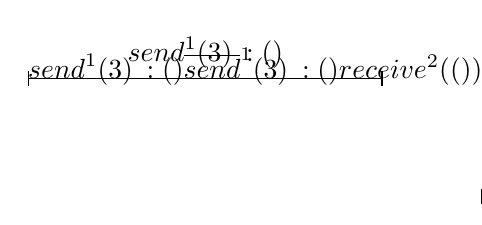
\begin{tikzpicture}[xscale = 0.9]
\draw[|-|] (0,0) -- node[above] {$\send^1(3)\::()$} (5,0);
\crossAt(1,0){$\send^1(3)\::()$}
\crossAt(4,0){$\overline{\send}^1(3)\::()$}
%\draw (1, 0) \X; \draw(4,0) \X;
\draw[|-|] (2,-1.5) -- node[above] {$\receive^2(())\::3$} (6,-1.5);
\crossAt(3,-1.5){$\receive^2(())\::3$}
%\draw(3,-1.5) \X;
\end{tikzpicture}
\end{center}

The definition of two-step linearisability then follows from this definition
of two-step compatability, precisely as in
Section~\ref{sec:specification-linearisability}.


%%%%%%%%%%%%%%%%%%%%%%%%%%%%%%%%%%%%%%%%%%%%%%%%%%%%%%%

\subsection{Proving the relationship}
\label{sec:twoStepLinSpec}

We now prove the relationship between synchronisation linearisation and
two-step linearisation.

Consider a synchonisation specification object |SyncSpec|.  We build a
corresponding two-step linearisation specification object~|TwoStepLinSpec|
such that synchronisation linearisation with respect to |SyncSpec| is
equivalent to two-step linearisation with respect to~|TwoStepLinSpec|.  The
definition we choose is not the simplest possible, but it is convenient for
the testing framework we use in Section~\ref{sec:testing-hacking}.  

The definition of |TwoStepLinSpec| is below.  We assume that each thread has
an identity in some range $\range 0 {\sm{NumThreads}}$.  For simplicity, we
arrange for this identity to be included in the $\call$ events written to the
log for operations~|op|\s1 and $\overline{\sm{op}}_1$.  (Alternatively, we
could implement thread identities internally to the object, for example using
the technique from~\cite[Appendix~A.2.4]{herlihy-shavit}.)

This object requires that corresponding invocations of~|op|\s1 and~|op|\s2 are
linearised consecutively: it does this by encoding the automaton on the right.
However, it allows the corresponding $\overline{\sm{op}}_1$ to be linearised
later (but before the next operation invocation by the same thread).  It uses
an array |returns|, indexed by thread identities, to record the value that
should be returned by an $\overline{\sm{op}}_1$ invocation by each thread.
Each invocation of $\op_2$ calls |SyncSpec.sync| to obtain the values that
should be returned for synchronisation linearisation; it writes the value for
the corresponding $\overline\op_1$ into |returns|.
%
\begin{trivlist}
\item[]
\begin{minipage}{92mm}
\begin{scala}
type ThreadID = Int               // Thread identifiers
val NumThreads: ThreadID = ... // Number of threads
trait State
case class Zero extends State
case class One(t: ThreadID, x£\s1£: A£\s1£) extends State
\end{scala}
\end{minipage}
%%%%%
\hfill 
%
\begin{minipage}{37.8mm}
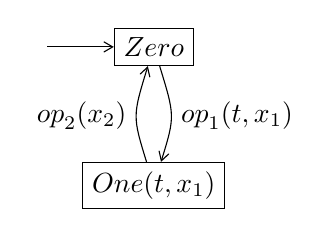
\begin{tikzpicture}[>= angle 60, xscale = 0.9, yscale = 0.44]
\draw (0,0) node[draw] (zero) {$\sm{Zero}$};
\draw[->] (zero) ++ (-1.5, 0) -- (zero);
%
\draw (0,-4) node[draw] (one) {$\sm{One}(\sm t, \sm{x}_1)$};
\draw[->] (zero) .. controls ++(0.3,-2) .. 
  node[right] {$\sm{op}_1(\sm t, \sm{x}_1)$} (one); 
%
\draw[->] (one) .. controls ++(-0.3,2) .. 
  node[left] {$\sm{op}_2(\sm x_2)$} (zero);
\end{tikzpicture}%
\end{minipage}%
%%%%%
\begin{scala}
object TwoStepLinSpec{
  private var state: State = Zero
  private val returns = new Array[Option[B£\s1£]](NumThreads)
  for(t <- 0 until NumThreads) returns(t) = None
  def op£\s1£(t: ThreadID, x£\s1£: A£\s1£): Unit = {
    require(state.isInstanceOf[Zero] && returns(t) == None); state = One(t, x£\s1£); ()
  }
  def op£\s2£(x£\s2£: A£\s2£): B£\s2£ = {
    require(state.isInstanceOf[One]); val One(t, x£\s1£) = state
    val (y£\s1£, y£\s2£) = SyncSpec.sync(x£\s1£, x£\s2£); returns(t) = Some(y£\s1£); state = Zero; y£\s2£
  }
  def £$\overline{\sm{op}}_1$£(t: ThreadID): B£\s1£ = {
    require(state.isInstanceOf[Zero] && returns(t).isInstanceOf[Some])
    val Some(y£\s1£) = returns(t); returns(t) = None; y£\s1£
  }
}
\end{scala}
\end{trivlist}

%%%%%

%% \framebox{Do we want to talk about \emph{complete} histories of
%%   TwoStepDelayedLinSpec?} -- containing all three events of a set

The following lemma identifies important properties of
|Two|\-|Step|\-|Delayed|\-|LinSpec|.  It follows immediately from the
definition.
%
\begin{lemma}
\label{lem:TwoStepLinSpec-histories}
Within any legal history of |TwoStepDelayedLinSpec|, events $\op_1$ and
$\op_2$ alternate.  Let $\op_1^{i_1}(t,x_1) \:: ()$ and $\op_2^{i_2}(x_2) \::
y_2$ be a consecutive pair of such events.  Then |op|\s2 makes a call
$\sm{SyncSpec.sync}(x_1, x_2)$ obtaining result $(y_1,y_2)$.  The next event
for thread~$t$ (if any) will be $\overline\op_1^{i_1}(t) \:: y_1$; and this
will be later in the history than $\op_2^{i_2}(x_2) \:: y_2$.  Further, the
corresponding history of events $\sm{sync}^{i_1,i_2}(x_1,x_2) \:: (y_1,y_2)$
is a legal history of |SyncSpec|.

Conversely, each history with events ordered in this way will be a legal
history of |TwoStepDelayedLinSpec| if  the corresponding history
of events $\sm{sync}^{i_1,i_2}(x_1,x_2) \:: (y_1,y_2)$ is a legal history of
|SyncSpec|.
\end{lemma}

%%%%%

The following proposition reduces synchronisation linearisability to two-step
linearisability.
%
\begin{prop}
Let |SyncObj| be a synchronisation object, |SyncSpec| be a synchronisation
specification object, and let |TwoStepLinSpec| be built from |SyncSpec| as
above.  Then |SyncObj| is two-step linearisable with respect to
|Two|\-|Step|\-|LinSpec| if and only if it is synchronisation linearisable
with respect to |SyncSpec|.
\end{prop}
%%%%%%
\begin{proof}
\textbf{($\implies$).}\quad
%
Let $h$ be a concurrent history of |SyncObj|.  By assumption, there is an
extension $h'$ of~$h$, and a legal history~$h_s$ of |TwoStepLinSpec| such that
$h'' = complete(h')$ and~$h_s$ are two-step-compatible.
%
Build a history~$h_s'$ of |SyncSpec| by replacing each consecutive pair
$\sm{op}_1^{i_1}(x_1) \:: ()$,\, $\sm{op}_2^{i_2}(x_2) \:: y_2$ in~$h_s$ by
the event $\sm{sync}^{i_1,i_2}(x_1,x_2) \:: (y_1,y_2)$, where $y_1$ is the
value returned by the corresponding~$\overline{\sm{op}}_1^{i_1}()$.
%
This is illustrated by the example timeline below, where $h''$ is represented
by the horizontal lines and the labels above; $h_s$ is represented by the
``$\cross$''s and the labels below; and $h_s'$ is represented by the
``$\bullet$'' and the label below.
%
\begin{center}
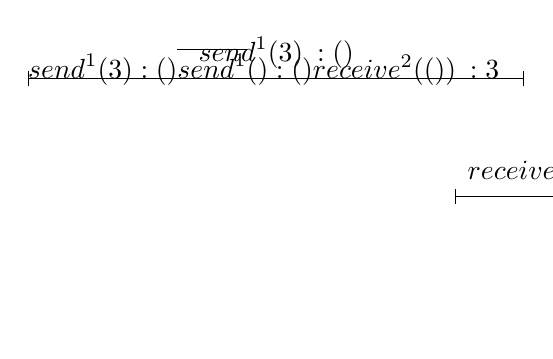
\begin{tikzpicture}[xscale = 0.9]
\draw[|-|] (0,0) -- node[above] {$\send^1(3)\::()$} (7,0);
\crossAt(1,0){$\send^1(3):()$}
%\draw (1, 0) \X; \draw (1,-0.4) node{$\sm{send}^1(3):()$}; 
\crossAt(6,0){$\overline{\send^1}():()$}
%\draw(6,0) \X; \draw(6,-0.4) node{$\overline{\sm{send}^1}():()$};
%
\draw[|-|] (2,-1.5) -- node[above] {$\receive^2(())\::3$} (5,-1.5);
\crossAt(3,-1.5){$\receive^2(())\::3$};
%\draw(3,-1.5) \X; \draw(3,-1.9) node{$\sm{receive}^2(())\::3$};
%
\draw(3,-2.5) node{$\bullet$}; 
\draw(3,-2.9) node{$\sm{sync}^{1,2}(3,()): ((),3)$};
\end{tikzpicture}
\end{center}

The history~$h_s'$ is legal for |SyncSpec| by
Lemma~\ref{lem:TwoStepLinSpec-histories}.
%
It is possible to interleave $h''$ and~$h_s'$ by placing each event
$\sm{sync}^{i_1,i_2}(x_1,x_2) \:: (y_1,y_2)$ in the same place as the
corresponding event $\sm{op}_2^{i_2}(x_2) \:: y_2$ in the interleaving
of~$h''$ and~$h_s$; by construction, this is between
$\call.\sm{op}_1^{i_1}(x_1)$ and~$\return.\sm{op}_1^{i_1} \:: y_1$, and
between $\call.\sm{op}_2^{i_2}(x_2)$ and~$\return.\sm{op}_2^{i_2} \:: y_2$.
%
Hence $h''$ and~$h_s$ are synchronisation-compatible; so $h''$ is
synchronisation-linearisable; and so $h$ is synchronisation-linearisable.

%%%%%

\textbf{($\Leftarrow$).}\quad
%
Let $h$ be a complete history of |SyncObj|.  By assumption, there is an
extension $h'$ of~$h$, and a legal history~$h_s$ of |SyncSpec| such that $h''
= complete(h')$ and~$h_s$ are synchronisation compatible.
%
Build a history~$h_s'$ of |TwoStepLinSpec| by replacing each event
$\sm{sync}^{i_1,i_2}(x_1,x_2) \:: (y_1,y_2)$ in~$h_s$ by the three consecutive
events $\sm{op}_1^{i_1}(x_1) \:: ()$,\, $\sm{op}_2^{i_2}(x_2) \:: y_2$,\,
$\overline{\sm{op}}_1^{i_1}() \:: y_1$.

The history~$h_s'$ is legal for |TwoStepLinSpec| by
Lemma~\ref{lem:TwoStepLinSpec-histories}.
%
It is possible to interleave $h''$ and~$h_s'$ by placing each triple
$\sm{op}_1^{i_1}(x_1) \:: ()$,\, $\sm{op}_2^{i_2}(x_2) \:: y_2$,\,
$\overline{\sm{op}}_1^{i_1}() \:: y_1$ in the same place as the corresponding
event $\sm{sync}^{i_1,i_2}(x_1,x_2) \:: (y_1,y_2)$ in the interleaving
of~$h''$ and~$h_s$; by construction, each $\sm{op}_1^{i_1}(x_1) \:: ()$ and
$\overline{\sm{op}}_1^{i_1}() \:: y_1$ are between
$\call.\sm{op}_1^{i_1}(x_1)$ and~$\return.\sm{op}_1^{i_1} \:: y_1$; and each
$\sm{op}_2^{i_2}(x_2) \:: y_2$ is between $\call.\sm{op}_2^{i_2}(x_2)$
and~$\return.\sm{op}_2^{i_2} \:: y_2$.
%
Hence $h''$ and~$h_s$ are two-step-compatible; so $h''$ is
two-step-linearisable; and so $h$ is two-step-linearisable.
\end{proof}

The two-step linearisation specification object can often be significantly
simplified from the template definition above.  Here is such a specification
object for a synchronous channel.
%
\begin{scala}
object SyncChanTwoStepLinSpec{
  private var state = 0           // Takes values 0, 1, cyclically 
  private var threadID = -1    // Current thread ID when state = 1
  private val canReturn =       // which senders can return?
    new Array[Boolean](NumThreads) 
  private var value: A = _      // The current value being sent
  def send(t: ThreadID, x: A): Unit = { 
    require(state == 0 && !canReturn(t)); value = x; threadID = t; state = 1 }
  def receive(u: Unit): A = { 
    require(state == 1); canReturn(threadID) = true; state = 0; value }
  def £$\overline{\send}$£(t: ThreadID): Unit = { 
    require(state == 0 && canReturn(t)); canReturn(t) = false }
}
\end{scala}

%%%%%%%%%%%%%%%%%%%%%%%%%%%%%%%%%%%%%%%%%%%%%%%%%%%%%%%

%% \subsection{Old version}

%% We now prove the relationship between synchronisation linearisation and
%% two-step linearisation.

%% Consider a synchonisation specification object |SyncSpec|.  We build a
%% corresponding two-step linearisation specification object~|TwoStepLinSpec|
%% such that synchronisation linearisation with respect to |SyncSpec| is
%% equivalent to two-step linearisation with respect to~|TwoStepLinSpec|.  The
%% definition is below: the specification's behaviour is described by the
%% automaton on the right.\footnote{Defining the subclasses of {\scalashape
%%     State} as {\scalashape case class}es allows pattern matching against such
%%   values.  For example, the statement {\scalashape val One(x}\s1{\scalashape )
%%     = state} succeeds only if {\scalashape state} has type {\scalashape One},
%%   and binds the name {\scalashape x}\s1 to the value of the {\scalashape x}\s1
%%   field of {\scalashape state}.}
%% \begin{trivlist}
%% \item[]
%% \begin{minipage}[b]{68mm}
%% \begin{scala}
%% trait State
%% case class Zero extends State
%% case class One(x£\s1£: A£\s1£) extends State
%% case class Two(y£\s1£: B£\s1£) extends State
%% \end{scala}
%% \end{minipage}
%% %
%% \hfil
%% %
%% \begin{minipage}[b]{63mm}
%% \begin{tikzpicture}[>= angle 60, xscale = 0.95, yscale = 0.75]
%% \draw (0,0) node[draw] (zero) {$\sm{Zero}$};
%% \draw[->] (zero) ++ (-1.5, 0) -- (zero);
%% %
%% \draw (4,0) node[draw] (one) {$\sm{One}(\sm{x}_1)$};
%% \draw[->] (zero)  -- node[above] {$\sm{op}_1(\sm{x}_1)$} (one); 
%% %
%% \draw (2, -2) node[draw] (two) {$\sm{Two}(\sm{y}_1)$};
%% \draw[->] (one)  -- node[right] {$\sm{op}_2(\sm{x}_2)$} (two); 
%% \draw[->] (two) -- node[left] {$\overline{\sm{op}}_1()$} (zero);
%% \end{tikzpicture}
%% \end{minipage}
%% %
%% %The specification object is defined as follows.
%% %
%% %% trait LinState
%% %% case class Zero extends LinState
%% %% case class One(x£\s1£: A£\s1£) extends LinState
%% %% case class Two(y£\s1£: B£\s1£) extends LinState
%% %
%% \begin{scala}
%% class TwoStepLinSpec{
%%   private var state: State = Zero
%%   def op£\s1£(x£\s1£: A£\s1£): Unit = {
%%     require(state.isInstanceOf[Zero]); state = One(x£\s1£)
%%   }
%%   def op£\s2£(x£\s2£: A£\s2£): B£\s2£ = {
%%     require(state.isInstanceOf[One]); val One(x£\s1£) = state
%%     val (y£\s1£, y£\s2£) = SyncSpec.sync(x£\s1£, x£\s2£); state = Two(y£\s1£); y£\s2£
%%   }
%%   def £$\overline{\sm{op}}_1$£(): B£\s1£ = {
%%     require(state.isInstanceOf[Two]); val Two(y£\s1£) = state; state = Zero; y£\s1£
%%   }
%% }
%% \end{scala}
%% \end{trivlist}
%% %
%% %
%% The definition forces the operations to take place in the order described by
%% the automaton.  In addition, the |op|\s2 operation calls the |sync| method on
%% |SyncSpec|, to calculate the return values and to update |SyncSpec|'s state;
%% it stores |op|\s1's result in the state. 

%% % in effect, the synchronisation happens at this point.

%% The following lemma follows immediately from the construction
%% of~|Two|\-|Step|\-|LinSpec|. 
%% %
%% \begin{lemma}
%% \label{lem:TwoStepLinSpec-historiesX}
%% Each history of~|TwoStepLinSpec| is the concatenation of triples of events of
%% the form $\sm{op}_1^{i_1}(x_1) \:: ()$,\, $\sm{op}_2^{i_2}(x_2) \:: y_2$,\,
%% $\overline{\sm{op}}_1^{i_1}() \:: y_1$  such that |SyncSpec| has a
%% corresponding legal history of events $\sm{sync}^{i_1,i_2}(x_1,x_2) \::
%% (y_1,y_2)$, and vice versa.
%% \end{lemma}

%% %%%%%

%% The following proposition reduces synchronisation linearisability to two-step
%% linearisability.
%% %
%% \begin{prop}
%% Let |SyncObj| be a synchronisation object, |SyncSpec| be a synchronisation
%% specification object, and let |TwoStepLinSpec| be built from |SyncSpec| as
%% above.  Then |SyncObj| is two-step linearisable with respect to
%% |Two|\-|Step|\-|LinSpec| if and only if it is synchronisation linearisable
%% with respect to |SyncSpec|.
%% \end{prop}
%% %%%%%%
%% \begin{proof}
%% \textbf{($\implies$).}\quad
%% %
%% Let $h$ be a concurrent history of |SyncObj|.  By assumption, there is an
%% extension $h'$ of~$h$, and a legal history~$h_s$ of |TwoStepLinSpec| such that
%% $h'' = complete(h')$ and~$h_s$ are two-step compatible.
%% %
%% Build a history~$h_s'$ of |SyncSpec| by replacing each triple
%% $\sm{op}_1^{i_1}(x_1) \:: ()$,\, $\sm{op}_2^{i_2}(x_2) \:: y_2$,\,
%% $\overline{\sm{op}}_1^{i_1}() \:: y_1$ in~$h_s$ by the event
%% $\sm{sync}^{i_1,i_2}(x_1,x_2) \:: (y_1,y_2)$.  
%% %
%% The history~$h_s'$ is legal by Lemma~\ref{lem:TwoStepLinSpec-histories}.  
%% %
%% It is possible to interleave $h''$ and~$h_s'$ by placing each event
%% $\sm{sync}^{i_1,i_2}(x_1,x_2) \:: (y_1,y_2)$ in the same place as the
%% corresponding event $\sm{op}_2^{i_2}(x_2) \:: y_2$ in the interleaving
%% of~$h''$ and~$h_s$; by construction, this is between
%% $\call.\sm{op}_1^{i_1}(x_1)$ and~$\return.\sm{op}_1^{i_1} \:: y_1$, and
%% between $\call.\sm{op}_2^{i_2}(x_2)$ and~$\return.\sm{op}_2^{i_2} \:: y_2$.
%% %
%% Hence $h''$ and~$h_s$ are synchronisation compatible, so $h''$ is
%% synchronisation lineariable, and so $h$ is synchronisation linearisable.

%% %%%%%

%% \textbf{($\Leftarrow$).}\quad
%% %
%% Let $h$ be a complete history of |SyncObj|.  By assumption, there is an
%% extension $h'$ of~$h$, and a legal history~$h_s$ of |SyncSpec| such that $h''
%% = complete(h')$ and~$h_s$ are synchronisation compatible.
%% %
%% Build a history~$h_s'$ of |TwoStepLinSpec| by replacing each event
%% $\sm{sync}^{i_1,i_2}(x_1,x_2) \:: (y_1,y_2)$ in~$h_s$ by the three events
%% $\sm{op}_1^{i_1}(x_1) \:: ()$,\, $\sm{op}_2^{i_2}(x_2) \:: y_2$,\,
%% $\overline{\sm{op}}_1^{i_1}() \:: y_1$.
%% %
%% The history~$h_s'$ is legal by Lemma~\ref{lem:TwoStepLinSpec-histories}.
%% %
%% It is possible to interleave $h''$ and~$h_s'$ by placing each triple
%% $\sm{op}_1^{i_1}(x_1) \:: ()$,\, $\sm{op}_2^{i_2}(x_2) \:: y_2$,\,
%% $\overline{\sm{op}}_1^{i_1}() \:: y_1$ in the same place as the corresponding
%% event $\sm{sync}^{i_1,i_2}(x_1,x_2) \:: (y_1,y_2)$ in the interleaving
%% of~$h''$ and~$h_s$; by construction, each $\sm{op}_1^{i_1}(x_1) \:: ()$ and
%% $\overline{\sm{op}}_1^{i_1}() \:: y_1$ are between
%% $\call.\sm{op}_1^{i_1}(x_1)$ and~$\return.\sm{op}_1^{i_1} \:: y_1$; and each
%% $\sm{op}_2^{i_2}(x_2) \:: y_2$ is between $\call.\sm{op}_2^{i_2}(x_2)$
%% and~$\return.\sm{op}_2^{i_2} \:: y_2$.
%% %
%% Hence $h''$ and~$h_s$ are two-step compatible, so $h''$ is two-step
%% lineariable, and so $h$ is two-step linearisable.
%% \end{proof}

%% %%%%%%%%%%

%% The two-step linearisation specification object can often be significantly
%% simplified from the template definition above.  Here is such a specification
%% object for a synchronous channel.
%% %
%% \begin{scala}
%% object SyncChanTwoStepLinSpec{
%%   private var state = 0        // Takes values 0, 1, 2, cyclically 
%%   private var value: A = _    // The current value being sent
%%   def send(x: A): Unit = { require(state == 0); value = x; state = 1 }
%%   def receive(u: Unit): A = { require(state == 1); state = 2; value }
%%   def £$\overline{\sm{send}}$£(): Unit = { require(state == 2); state = 0 }
%% }
%% \end{scala}

%%%%%%%%%%%%%%%%%%%%%%%%%%%%%%%%%%%%%%%%%%%%%%%%%%%%%%%

\subsection{Synchronising more than two operations}
\label{ssec:relating-variations}

The results of the previous subsections carry across to non-binary
synchronisations, in a straightforward way.  For a synchronisation object with
$k$ operations, |op|\s1, \ldots, |op|$_k$, the corresponding two-step
linearisation specification object has $2k-1$ operations, |op|\s1, \ldots,
|op|$_k$, $\overline{\sm{op}}_1$, \ldots, $\overline{\sm{op}}_{k-1}$.  The
definition of two-step linearisation is then the obvious adaptation of the
binary case: each operation |op|\s{i} of the synchronisation object is
linearised by the composition of |op|\s{i} and $\overline{\op}_i$ of the
specification object, for $i = 1, \ldots, k-1$.

%% Each of the first $k - 1$ |op| operations takes a thread identity as a
%% parameter.

The construction of the previous subsection is easily adapted to the case of
$k$-way synchronisations for $k > 2$.  The specification object encodes an
automaton with $k$ states.  The figure below gives the automaton in the case
$k = 4$.
%
\begin{center}
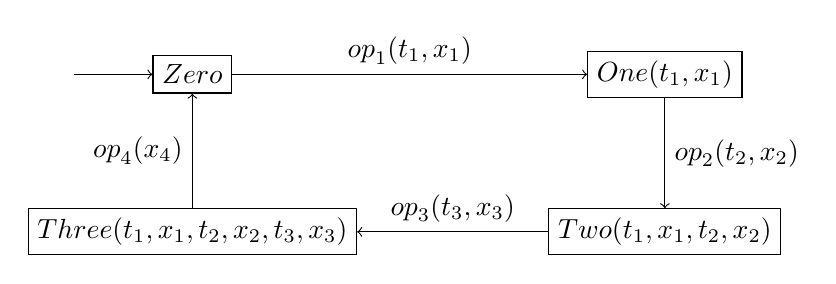
\begin{tikzpicture}[xscale = 1]
\draw (0,0) node[draw] (zero) {$\sm{Zero}$};
\draw[->] (zero) ++ (-1.5, 0) -- (zero);
%
\draw (zero)++(6,0) node[draw] (one) {$\sm{One}(\sm{t}_1, \sm{x}_1)$};
\draw[->] (zero)  -- node[above] {$\sm{op}_1(\sm{t}_1, \sm{x}_1)$} (one); 
%
\draw (one)++(0, -2) node[draw] (two) 
  {$\sm{Two}(\sm{t}_1, \sm{x}_1, \sm{t}_2, \sm{x}_2)$};
\draw[->] (one)  -- node[right] {$\sm{op}_2(\sm{t}_2, \sm{x}_2)$} (two); 
%
\draw (two)++(-6, 0) node[draw] (three) 
  {$\sm{Three}(\sm{t}_1, \sm{x}_1, \sm{t}_2, \sm{x}_2, \sm{t}_3, \sm{x}_3)$};
\draw[->] (two)  -- node[above] {$\sm{op}_3(\sm{t}_3, \sm{x}_3)$} (three); 
%
%% \draw (three)++(0,-2) node[draw] (threeX) 
%%   {$\sm{ThreeX}(\sm{y}_1, \sm{y}_2, \sm{y}_3)$};
\draw[->] (three)  -- node[left] {$\sm{op}_4(\sm{x}_4)$} (zero); 
%
%% \draw (threeX)++(-4,0) node[draw] (twoX) {$\sm{TwoX}(\sm{y}_1, \sm{y}_2)$};
%% \draw[->] (threeX)  -- node[above] {$\overline{\sm{op}}_3()$} (twoX); 
%% %
%% \draw (twoX)++(-3.5,0) node[draw] (oneX) {$\sm{OneX}(\sm{y}_1)$};
%% \draw[->] (twoX)  -- node[above] {$\overline{\sm{op}}_2()$} (oneX);
%% \draw [->] (oneX)  -- node[below] {$\overline{\sm{op}}_1()$} (zero);
\end{tikzpicture}
\end{center}
%
The final |op| operation, |op|\s4 in the above figure, applies the |sync|
method of the synchronisation specification object to the parameters $\sm x_1,
\ldots, \sm x_k$ to obtain the results $\sm y_1, \ldots, \sm y_k$; it stores
the first $k-1$ in appropriate |returns|\s{i} arrays, and returns $\sm y_k$
itself.  In the case $k=4$, it has definition:
%
\begin{scala}
  def op£\s4£(x£\s4£: A£\s4£): B£\s4£ = {
    require(state.isInstanceOf[Three]); val Three(t£\s1£, x£\s1£, t£\s2£, x£\s2£, t£\s3£, x£\s3£) = state
    val (y£\s1£, y£\s2£, y£\s3£, y£\s4£) = SyncSpec.sync(x£\s1£, x£\s2£, x£\s3£, x£\s4£) 
    returns£\s1£(t£\s1£) = Some(y£\s1£); returns£\s2£(t£\s2£) = Some(y£\s2£); returns£\s3£(t£\s3£) = Some(y£\s3£)
    state = Zero; y£\s4£
  }
\end{scala}
%
Each $\overline{\sm{op}}_i$ operation retrieves the result from the
corresponding |returns|\s{i} array.
 % relating synchronisation linearisation and linearisation
\section{Linearisability testing}
\label{sec:lin-testing}

In the following two sections, we describe techniques for testing whether the
implementation of a synchronisation object is synchronisation linearisable
with respect to a synchronisation specification object.
%
The techniques are influenced by the techniques for testing (standard)
linearisation~\cite{gavin:lin-testing}, so we begin by sketching those
techniques.

The idea of linearisability testing is as follows.  We run several
\emph{worker threads}, performing operations (typically chosen randomly) upon
the concurrent datatype that we are testing, and logging the calls and
returns.  More precisely, a thread that performs a particular
operation~$\sm{op}^i(x)$: (1) writes $\call.\sm{op}^i(x)$ into the log;
(2)~performs $\sm{op}(x)$ on the synchonisation object, obtaining result~$y$,
say; (3)~writes $\return.\sm{op}^i \:: y$ into the log.  Further, the logging
associates each operation execution with an execution $\sm{op}(x)$ of the
corresponding operation on the specification object.

Once all worker threads have finished, we can use an algorithm to test whether
the history is linearisable with respect to the specification object.  The
algorithm searches for an order to linearise the executions, consistent with
what is recorded in the log, and such that the order represents a legal
history of the corresponding executions on the specification object.
See~\cite{gavin:lin-testing} for details of several algorithms.

This process can be repeated many times, so as to generate and analyse many
histories.  Our experience is that the technique works well.  It seems
effective at finding bugs, where they exist, typically within a few seconds;
for example, we used it to find an error in the concurrent priority queue
of~\cite{faulty-pri-queue}, which we believe had not previously been
documented.  Further, the technique is easy to use: we have taught it to
undergraduate students, who have used it effectively.

Note that this testing concentrates upon the safety property of
linearisability, rather than liveness properties such as deadlock-freedom.
However, if the concurrent object can deadlock, it is likely that the testing
will discover this.  Related to this point, it is the responsibility of the
tester to define the worker threads in a way that all executions will
eventually return, so the threads terminate.  For example, consider a partial
stack where a |pop| operation blocks while the stack is empty; here, the
tester would need to ensure that threads collectively perform at least as many
|push|es as |pop|s, to ensure that each |pop| does eventually return.

Note also that there is potentially a delay between a worker thread writing the
$\call$ event into the log and actually calling the operation; and likewise
there is potentially a delay between the operation returning and the thread
writing the $\return$ event into the log.  However, these delays do not
generate false errors: if a history without such delays is linearisable, then
so is a corresponding history with delays.  We believe that it is essential
that the technique does not give false errors: an error reported by testing
should represent a real error; testing of a correct implementation should be
able to run unsupervised, maybe for a long time.  Further, our experience is
that the delays do not prevent the detection of bugs when they exist (although
might require performing the test more times).  This means that a failure to
find any bugs, after a large number of tests, can give us good confidence in
the correctness of the concurrent datatype.

%%%%%%%%%%%%%%%%%%%%%%%%%%%%%%%%%%%%%%%%%%%%%%%%%%%%%%%

\section{Hacking the linearisablity framework}
\label{sec:testing-hacking}

In this section we investigate how to use the existing linearisation testing
framework for testing synchronisation linearisation, using the ideas of
Section~\ref{sec:relating}.  This is not a use for which the framework
was intended, so we consider it a hack.  However, it has the advantage of not
requiring the implementation of any new algorithms.  (We do not consider
progressibility in this section.)

Recall, from the introduction of Section~\ref{sec:relating}, that a
straightforward approach won't work.  Instead we adapt the idea of two-step
linearisation from later in that section.  We start by considering the case of
binary heterogeneous synchronisation.  We aim to obtain a log history that can
be tested for (standard) linearisability against |TwoStepLinSpec|.

As with standard linearisability testing, we run several worker threads,
calling operations on the synchronisation object, and logging the calls and
returns.
%
\begin{itemize}
\item A thread~$t_1$ that performs the concrete operation~$\op_1(x_1)$:
  (1)~writes $\call.\sm{op}_1^{i_1}(x_1)$ into the log, associating it with a
  corresponding execution $\op_1(t_1, x_1)$ on the specification object;
  (2)~performs $\op_1(x_1)$ on the synchonisation object, obtaining
  result~$y_1$, say; (3)~writes $\return.\op_1^{i_1} \:: ()$ into the log;
  (4)~writes $\call.\overline{\op}_1^{i_1}()$ into the log, associating it
  with a corresponding execution $\overline{\op}_1(t)$ on the specification
  object; (5)~writes $\return.\overline{\op}_1^{i_1} \:: y_1$ into the log.

\item A thread~$t_2$ that performs operation~|op|\s2, acts as for standard
  linearisability testing.  It: (1)~writes $\call.\sm{op}_2^{i_2}(x_2)$ into
  the log, associating it with a corresponding execution $\op_2(x_2)$ on the
  specification object; (2)~performs $\op_2(x_2)$ on the synchonisation
  object, obtaining result~$y_2$, say; (3)~writes $\return.\op_2^{i_2} \::
  y_2$ into the log
\end{itemize}
%
The top half of Figure~\ref{fig:twostep-timeline} illustrates a possible run,
containing a single synchronisation, together with the log history.

\begin{figure}
\begin{center}
\def\y{-1.4} % op_2 y-coord
\def\ySLin{-2.5} % sync-lin y-ccord
\def\yLin{-3.6} % linearisation y-coord
\begin{tikzpicture}%[yscale = 1.4]
\bulletAt(-0.6,0){$\call.\op_1(x_1)$};
\draw[|-|] (0.0,0) -- node[above] {$\op_1(x_1)\::y_1$} (2.5,0);
\bulletAt(3.0,0){$\return.\op_1$};
\bulletAt(4.7,0){$\call.\overline{\op}_1$};
\bulletAt(6.5,0){$\return.\overline{\op}_1\::y_1$};
%
\bulletAt(-0.3,\y){$\call.\op_2(x_2)$};
\draw[|-|] (0.2,\y) -- node[above]{$\op_2(x_2)\::y_2$} (2.6,\y);
\bulletAt(3.2,\y){$\return.\op_2\::y_2$};
%
\draw (-2,\ySLin) node{$h_s$};
\crossAt(1.4,\ySLin){$\sync(x_1,x_2)\::(y_1,y_2)$};
%
\draw (-2,\yLin) node{$h_{2s}$:};
\draw(1.2,\yLin) \X; 
\draw(0.5,\yLin-0.4) node{\footnotesize $\op_1(t_1,x_1)$};
\draw(1.6,\yLin) \X;
\draw(2.3,\yLin-0.4) node{\footnotesize $\op_2(x_2)\::y_2$};
%% \crossAt(0.5,\yLin){$\op_1(t_1,x_1)$};
%% \crossAt(2.3,\yLin){$\op_2(x_2)\::y_2$};
\crossAt(5.5,\yLin){$\overline{\op}_1(t_1)\::y_1$};
\end{tikzpicture}
\end{center}
\caption{Illustration of two-step linearisation testing.  The operation
  executions are represented by the horizontal lines with labels above
  (denoted ``$h$'' in Proposition~\ref{prop:twostep-testing}).  The log
  entries are represented by the bullets with labels below (denoted ``$h_l$''
  in Proposition~\ref{prop:twostep-testing}).  Linearisation points are
  represented by crosses with labels below: the penultimate row, labelled
  ``$h_s$'', is a synchronisation linearisation; the bottom row, labelled
  ``$h_{2s}$'', is a linearisation of the two-step synchronisation object.
  Execution identifiers and null arguments and returns are omitted, for
  clarity.}
\label{fig:twostep-timeline}
\end{figure}

%%%%%

The following definition captures that a log history~$h_l$ might arise from a
concrete history~$h$, using the logging strategy described above.
%
\begin{definition}
Let $h$ be a complete history of a binary heterogeneous synchronisation
object, and let $h_l$ be a log history for the same object.  We say that the
two histories \emph{correspond} if there is some way of interleaving them such
that
%
\begin{itemize}
\item Each $\call.\op_1^{i_1}(x_1)$, from $h_l$, precedes the call and return
  of~$\op_1^{i_1}(x_1)\::y_1$ from~$h$, which precedes $\return.\op_1^{i_1} \::
  ()$, $\call.\overline{\op}_1^{i_1}()$ and $\return.\overline{\op}_1^{i_1}
  \:: y_1$, from~$h_l$, in that order.

\item Each $\call.\op_2^{i_2}(x_2)$, from $h_l$, precedes the call and return
  of~$\op_2^{i_2}(x_2)\::y_2$ from~$h$, which precedes $\return.\op_2^{i_2}
  \:: y_2$, from~$h_l$.
\end{itemize}
\end{definition}

%%%%%

As with standard linearisation, the tester needs to define the worker threads
so that all executions will eventually return, i.e.~that each will be able to
synchronise.  For a binary heterogeneous synchronisation with no precondition,
we can achieve this by half the threads calling one operation, and the other
half calling the other operation (with the same number of calls by each).  For
a binary homogeneous synchronisation, this approach might not work if every
worker does more than one operation: one worker might end up with two
operations to perform, when all others have terminated; instead, we arrange
for an even number of workers to each perform one operation. 

Once all threads have finished, we test whether the log history is
linearisable (i.e.~standard linearisation) with respect to |TwoStepLinSpec|
from Section~\ref{sec:relating}.  Figure~\ref{fig:twostep-timeline} gives an
example linearisation. 

Note that we have three related concepts here: (1)~synchronisation
linearisation of the concrete history of operation executions with respect to
|SyncSpec|; (2)~two-step linearisation of the concrete history with respect
to~|TwoStepLinSpec|; and (3)~linearisation of the log history with respect
to~|TwoStepLinSpec|.  Proposition~\ref{prop:two-step-lin} shows that the first
two of these are equivalent.  We need to show that these imply~(3), so the
technique does not give false errors.  (The converse might not hold, because
of delays in writing to the log.)

\begin{prop}
\label{prop:twostep-testing}
Let $h$ be a complete history of a binary heterogeneous synchronisation
object, and let $h_l$ be a corresponding log history for the same object.  Let
|SyncSpec| be a synchronisation specification object, and |TwoStepSyncSpec|
the corresponding two-step synchronisation specification object, constructed
as in Section~\ref{sec:twoStepLinSpec}.  Suppose $h$ is synchronisation
linearisable with respect to |SyncSpec|.  Then $h_l$ is linearisable with
respect to |TwoStepSyncSpec|.
\end{prop}
%
\begin{proof}
Since $h$ is synchronisation linearisable, there is a legal history~$h_s$ of
|SyncSpec| such that $h_s$ is a synchronisation linearisation of $h$.
Consider the interleaving of $h_s$ and~$h$, that demonstrates this, and
interleave $h_l$ with it, consistent with the interleaving of~$h$ and~$h_l$
that demonstrates that they correspond.  Figure~\ref{fig:twostep-timeline}
illustrates such an interleaving.

We build a history~$h_{2s}$ of~|TwoStepSyncSpec|, and interleave it with~$h_l$
as follows.  In the interleaving of the previous paragraph, replace each event
$\sync^{i_1,i_2}(x_1,x_2)\::(y_1,y_2)$ (from~$h_s$) by consecutive
events~$\op_1^{i_1}(x_1)\::()$ and $\op_2^{i_2}(x_2)\::y_2$, and add
$\overline{\op}_1^{i_1}()\::y_1$ between $\call.\overline{\op}_1^{i_1}()$ and
$\return.\overline{\op}_1^{i_1} \:: y_1$ (from~$h_l$).  Again,
Figure~\ref{fig:twostep-timeline} illustrates such an interleaving.  This is a
legal history of~|TwoStepSyncSpec|, by
Lemma~\ref{lem:TwoStepLinSpec-histories}.  Further, each event of~$h_{2s}$ is
between the corresponding $\call$ and $\return$ events of~$h_l$, by
construction.  Hence $h_{2s}$ is a linearisation of~$h_l$.
\end{proof}

%%%%%%%%%%%%%%%%%%%%%%%%%%%%%%%%%%%%%%%%%%%%%%%%%%%%%%%

%% \subsection{OLD VERSION}

%% Note there might be delays involved in writing to the log, so that the log
%% history does not correspond precisely to the history of operation calls and
%% returns.  We show that the approximation serves our purposes.

%% Consider a history~$h$ of the synchronisation object, and suppose, for the
%% moment, there are no delays in logging, i.e.:\ (1)~the $\call.\op_1$ and
%% $\call.\op_2$ events happen immediately before the actual calls; (2)~the
%% $\return.\op_2$ events happen immediately after the return of~$\op_2$; and
%% (3)~the $\call.\overline\op_1$ and $\return.\overline\op_1$ events happen
%% immediately after the return of $\op_1$ --- in each case with no intervening
%% events.  Then the log history is linearisable with respect to |TwoStepLinSpec|
%% if and only if the history~$h$ is two-step linearisable with respect to
%% |TwoStepLinSpec|.  But Proposition~\ref{prop:two-step-lin} then shows that
%% this holds if and only if $h$ is synchronisation linearisable.  In particular,
%% this shows that errors are detected providing the logging is fast enough.

%% We now show that delays in logging do not introduce false errors.  Consider a
%% history~$h$ that is synchronisation linearisable, and consider the
%% corresponding log history~$h_l$.  Now build a history~$h'$ so that each
%% operation is extended so that: (1)~each call of~$\op_1$ or~$\op_2$ is
%% immediately before the $\call.\op_1$ or $\call.\op_2$ event in~$h_l$; (2)~each
%% return of~$\op_1$ is immediately after the $\return.\overline\op_1$ event
%% in~$h_l$; and (3)~each return of~$\op_2$ is immediately after the
%% $\return.\op_2$ event in~$h_l$.  This construction is illustrated below for
%% the two types of operation.
%% %
%% \begin{center}
%% \begin{tikzpicture}[xscale = 1.0, yscale = 1.0]
%% \draw (-2.0,0) node{$h$:};
%% \draw (-2.0,-1) node{$h_l$:};
%% \draw (-2.0,-2.3) node{$h'$:};
%% % op_1^1
%% \draw[|-|] (0,0) -- node[above] {$\sm{op}_1(x_1)\::y_1$} (1,0);
%% \bulletAt(-0.2,-0.8){$\call.\sm{op}_1$}
%% \bulletAt(1.2,-0.8){$\return.\sm{op}_1$}
%% \bulletAt(2.7,-0.8){$\call.\overline{\op}_1$}
%% \bulletAt(4.2,-0.8){$\return.\overline{\op}_1$}
%% \draw[|-|] (-0.4,-2.3) -- node[above] {$\sm{op}_1(x_1)\::y_1$} (4.4,-2.3);
%% %%%%%
%% \draw[|-|] (7.0,0) -- node[above] {$\sm{op}_2(x_2)\::y_2$} (8,0);
%% \bulletAt(6.8,-0.8){$\call.\sm{op}_2$}
%% \bulletAt(8.2,-0.8){$\return.\op_2$}
%% \draw[|-|] (6.6,-2.3) -- node[above] {$\sm{op}_2(x_2)\::y_2$} (8.4,-2.3);
%% \end{tikzpicture}
%% \end{center}
%% %
%% Now $h$ is synchronisation linearisable; and hence $h'$ is also (since each
%% operation in $h'$ is an extension of the corresponding operation in~$h$).  But
%% then Proposition~\ref{prop:two-step-lin} implies that $h'$ is two-step
%% linearisable with respect to |TwoStepLinSpec|.  Hence $h_l$ is linearisable
%% with respect to |TwoStepLinSpec|, by construction.

This approach generalises to non-binary synchronisations, homogeneous
synchronisations, and stateful specification objects as in
Section~\ref{ssec:relating-variations}.

%\framebox{Generalisations}

%%%%%%%%%%%%%%%%%%%%%%%%%%%%%%%%%%%%%%%%%%%%%%%%%%%%%%%

% \framebox{Improve below}

\paragraph{Variable-arity synchronisations.}

It turns out that it is not, in general, possible to capture variable-arity
synchronisations using this technique, in particular where the arity of a
synchronisation depends upon the relative timing of executions, as opposed to
the state of the specification object.  This is a result of two things: that
the logging of operations, in particular the $\overline{\op}_1$, can be
arbitrarily delayed; and that it can be nondeterministic whether or not two
executions synchronise, which is at odds with the fact that each operation on
the specification object needs to be deterministic.

To illustrate this point, consider a timeout channel.  Without loss of
generality, let the |send| operation correspond to $\op_1$, and the
|receive| operation correspond to~$\op_2$.

The top-half of Figure~\ref{fig:two-step-timeout-channel} gives a
timeline illustrating a successful |send(3)| and |receive|.  Note that this
corresponds to the history
\[
\seq{ \send(3)\::(),\; \receive()\::\sm{Some}(3),\; 
  \overline{\send}(3)\::\sm{true} }
\]
of the specification object.

%%%%%%%%%%

\begin{figure}
\begin{center}
\def\yLin{-2.5} % y-coord for linearisation
\begin{tikzpicture}[xscale = 0.9]
\bulletAt(-0.4,0){$\call.\send(3)$};
\draw[|-|] (0,0) -- node[above] {$\send(3)\::()$} (1.6,0);
\bulletAt(2.0,0){$\return.\send$};
%
\bulletAt(3.9,0){$\call.\overline{\send}$};
\bulletAt(6.2,0){$\return.\overline{\send}\::\sm{true}$};
%
\bulletAt(-0.5,-1.5){$\call.\receive\qquad$};
\draw[|-|] (0.3,-1.5) -- 
  node[above] {$\receive()\::\sm{Some}(3)$} (1.9,-1.5);
\bulletAt(2.8,-1.5){\ $\qquad\qquad\return.\receive\::\sm{Some(3)}$};
%
\draw(0.7,\yLin) \X; 
\draw(-0.1,\yLin-0.4) node{\footnotesize $\send(3)\::()$};
\draw(1.1,\yLin) \X;
\draw(2.6,\yLin-0.4) node{\footnotesize $\receive()\::\sm{Some}(3)$};
%% \crossAt(0.7,-3){$\send(3)\::()$}
%% \crossAt(1.5,-3){$\receive()\::\sm{Some}(3)$}
\crossAt(5.5,\yLin){$\overline{\send}\::\sm{true}$}
%
\draw (-2,-3.4) -- ++(10,0); 
\end{tikzpicture}

%%%%%%
%\hfil\hfil
%\bigskip

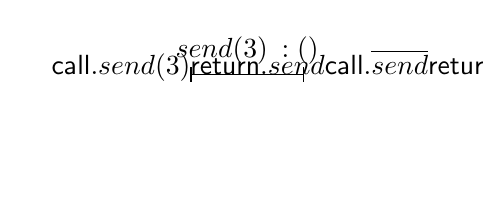
\begin{tikzpicture}[xscale = 0.9]
\bulletAt(-0.4,0){$\call.\send(3)$};
\draw[|-|] (0,0) -- node[above] {$\send(3)\::()$} (1.6,0);
\bulletAt(2.0,0){$\return.\send$};
%
\bulletAt(7.1,0){$\call.\overline{\send}$};
\bulletAt(9.4,0){$\return.\overline{\send}\::\sm{false}$};
%
\bulletAt(2.5,-1.5){$\call.\receive\qquad$};
\draw[|-|] (3.3,-1.5) -- 
  node[above] {$\receive()\::\sm{None}$} (4.9,-1.5);
\bulletAt(5.8,-1.5){\ $\qquad\qquad\return.\receive\::\sm{None}$};
%
\crossAt(0.8,\yLin){$\send(3)\::()$};
\crossAt(3.9,\yLin){$\receive()\::\sm{Some}(3)$};
\crossAt(8.2,\yLin){$\overline{\send}\::\sm{true}$}
%% \draw[|-|] (0,-3.5) -- node[above] {$\send(3)\::()$} (1.6,-3.5);
%% \crossAt(0.7,-3.5){$\send(3)\::()$}
%% %
%% \draw[|-|] (2.2,-5) -- 
%%   node[above] {$\receive()\::\sm{None}$} (3.8,-5);
%% \crossAt(3.4,-5){$\receive()\::\sm{Some}(3)$}
%% %
%% \draw[|-|] (4.0,-3.5) -- node[above] 
%%   {$\overline{\send}(3)\::\sm{false}$} (5.6,-3.5);
%% \crossAt(4.8,-3.5){$\overline{\send}(3)\::\sm{true}$}
\end{tikzpicture}
\end{center}
\caption{Figure showing why two-step linearisation cannot be used for a
  timeout channel.  Conventions are as in Figure~\ref{fig:twostep-timeline}.}
\label{fig:two-step-timeout-channel}
\end{figure}

%%%%%%%%%%

The bottom-half side of Figure~\ref{fig:two-step-timeout-channel} gives a
timeline illustrating an unsuccessful |send(3)| and |receive|, and where the
logging of $\overline{\send}$ is delayed.  None of the executions overlap, so
they must necessarily be linearised in the same order as in the previous
history.  The specification object is deterministic, so the operations must
return the same results as in the previous history.  But, in the cases of
$\receive$ and $\overline{\send}$, those returned values do not agree with the
corresponding values in the log history.  Hence the history would be flagged
as an error, despite being valid.

The difference between this situation and the discussion in
Section~\ref{ssec:relating-variations} concerns the fact that the logging of
operations, in particular the $\overline{\send}$, can be arbitrarily delayed.
However, in the earlier section we allowed the $\overline{\send}$ anywhere
within the corresponding concrete operation.  This means that a history like
in the bottom-half of Figure~\ref{fig:two-step-timeout-channel} could be
linearised by the history
\[
\seq{ \send(3)\::(),\; \overline{\send}(3)\::\sm{false},\;
  \receive()\::\sm{None} }
\]
of the two-step specification object, where the operations take place in a
different order than for Figure~\ref{fig:two-step-timeout-channel}; this is
consistent with a deterministic specification object.

A similar problem arises with a timeout exchanger.

%\framebox{Explain how it can be done.}

We have investigated an alternative approach, which involves worker threads
adapting their logging behaviour based on the outcome of their operations.
For the timeout channel:
\begin{itemize}
\item A thread that sends a value~$x$: (1)~writes $\call.\send^{i_1}(x)$ into
  the log; (2)~performs $\send(x)$ on the channel; (3)~writes
  $\return.\send^{i_1} \:: ()$ into the log; (4)~if the send is successful,
  associates the log entries with an operation $\send(x)$ on the specification
  object, and otherwise associates them with an operation $\sm{sendFail}(x)$;
  (5)~if the send is successful, writes $\call.\overline{\send}^{i_1}()$ and
  $\return.\overline{\send}_1^{i_1} \:: ()$ into the log, associating them
  with an operation $\overline{\send}()$ on the specification object (and
  otherwise does nothing).

%%     (6)~writes $\return.\overline{\send}_1^{i_1} \:: ()$ into the log

%% then:
%%   \begin{itemize}
%%   \item if the send is successful: (4) associates the log entries with an
%%     operation $\send(x)$ on the specification object; (5)~writes
%%     $\call.\overline{\send}^{i_1}()$ into the log, associating it with a
%%     corresponding execution $\overline{\send}()$ on the specification object;
%%     (6)~writes $\return.\overline{\send}_1^{i_1} \:: ()$ into the log.

%%   \item if the send is unsuccessful: (4)~associates the log entries with an
%%     operation $\sm{sendFail(x)}$ on the specification object (and does not
%%     perform the second step).
%%   \end{itemize}

\item A thread that performs a receive: (1)~writes $\call.\receive^{i_2}$ into
  the log; (2)~performs $\receive$ on the channel, receiving result~$r$, say;
  (3)~writes $\return.\receive^{i_1} \:: r$ into the log; (4)~if the receive
  was successful, associates the log entries with an operation |receive| on
  the specification, and otherwise associates them with an
  operation $\sm{receiveFail}$.
\end{itemize}


The specification object encodes the automaton below. 
%% \begin{window}[0,r,{
%% \begin{minipage}{73mm}
\begin{center}
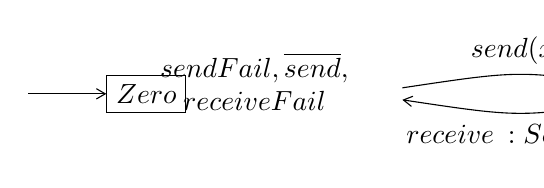
\begin{tikzpicture}[>= angle 60]
\draw (0,0) node[draw] (zero) {$\sm{Zero}$};
\draw[<-] (zero) -- ++ (-1.5,0);
\loopAbove(zero){$
%% \draw[->] (zero) .. controls ++(1.5,0.4) and (1.5,-0.4) .. node[right] {$
  \begin{array}{c} 
  \sm{sendFail}, \overline{\send}, \\ \sm{receiveFail}
  \end{array}$}% (zero);
%
\draw (4,0) node[draw] (one) {$\sm{One}(\sm{x})$};
\draw[->] (zero) .. controls ++(2,0.3) .. node[above] {$\sm{send(x)}$} (one); 
\draw[->] (one) .. controls ++(-2,-0.3) .. 
  node[below] {$\sm{receive}\::\sm{Some(x)}$} (zero);
\end{tikzpicture}
\end{center}
%% \end{minipage}
%% },] 
Thus a successful synchronisation is linearised by a sequence $\send(\sm x)$,
$\receive\::\sm{Some(x)}$, $\overline{\send}$, with the former two events
consecutive, as for other binary heterogeneous synchronisations.  Unsuccessful
sends and receives are each linearised by a single event.

A similar technique can be used for a timeout exchanger.  We consider this
approach convoluted, and we do not advocate it.  We include it only for
completeness.

 % testing algorithms
\section{Direct testing of synchronisation linearisation}
\label{sec:direct}

We now consider how to test for synchronisation linearisation more directly.
We perform logging precisely as for standard linearisation: a thread that
performs a particular operation~$\sm{op}^i(x)$: (1) writes
$\call.\sm{op}^i(x)$ into the log; (2)~performs $\sm{op}(x)$ on the
synchonisation object, obtaining result~$y$, say; (3)~writes
$\return.\sm{op}^i \:: y$ into the log.  

When not testing for progress, we make it the responsibility of the tester to
define the threads in a way that ensures that all invocations will be able to
synchronise, so all threads will eventually terminate.  For example, for a
binary heterogeneous synchronisation object, threads collectively should
perform the same number of each operation. 

When testing for progress, we remove the requirement on the tester to ensure
that all invocations can synchronise.  Indeed, in some cases, in order to find
failures of progress, it is necessary that not all invocations can
synchronise: we have examples of incorrect synchronisation objects where (for
example) if there are two invocations of $\op_1$ and one of~$\op_2$, then
\emph{neither} invocation of~$\op_1$ returns, signifying the failure of
progressability; but if there were a second invocation of~$\op_2$, it would
unblock both invocations of~$\op_1$, so all invocations would return, and the
failure of progressability would be missed.

Instead, we run threads performing operations, typically chosen at random; and
after a suitable duration, we interrupt any threads that have not yet
returned.  The duration before the interrupts needs to be chosen so that it is
highly likely that any threads that have not returned really are stuck:
otherwise this approach it likely to produce false positives.  In practice, we
have found it easy to identify a suitable duration.  A downside of this
approach is that the duration needs to be chosen fairly conservatively, which
increases the time that a given number of runs will take.

In the remainder of this section we consider algorithms for determining if the
resulting log history is synchronisation linearisable, and whether it also
satisfies progressability.  In Section~\ref{sec:algorithm-dfs} we present a
general algorithm for this problem, based on depth-first search.  We then
consider the complexity of this problem.  We show, in
Section~\ref{sec:NP-complete}, that the problem of deciding whether a history
is synchronisation linearisable is NP-complete in general.  However, we show
that in the case of binary synchronisations with a stateless specification
object the problem can be solved in polynomial time: we consider the
heterogeneous case in Section~\ref{sec:binary-heterogeneous}, and the
homogeneous case in Section~\ref{sec:binary-homogeneous}.  Nevertheless, in
Section~\ref{sec:non-binary-stateless} we show that for synchronisations of
three or more invocations, the problem is again NP-complete, even in the
stateless case.

%%  It turns out that the appropriate
%% algorithm, and corresponding complexity results, differ depending upon the
%% nature of the synchronisation object: whether synchronisations are binary, or
%% may involve more than two threads; and whether the object is stateful or
%% stateless. 

%% Main ideas: general algorithm; NP-complete in general case; quadratic in
%% stateless binary heterogeneous case; polynomial in binary homogeneous case;
%% NP-complete for synchronisations of arity more than~2 even in stateless case


%%%%%%%%%%%%%%%%%%%%%%%%%%%%%%%%%%%%%%%%%%%%%%%%%%%%%%%%%%%%

\subsection{The general case}
\label{sec:algorithm-dfs}

We describe an algorithm for deciding whether a given complete history~$h$ is
synchronisation linearisable with respect to a given synchronisation
specification object.  We transform the problem into a graph-search algorithm
as follows.

We define a search graph, where each node is a \emph{configuration}
comprising:
%
\begin{itemize}
\item An index $i$ into the log;

\item A set $pending$ of operation invocations that were called in the
  first~$i$ events of the log and that have not yet been linearised;

\item A set $linearised$ of operation invocations that were called in the
  first~$i$ events of the log and that have been linearised, but have not yet
  returned;

\item The state $spec$ of the specification object after the synchronisations
  linearised so far.
\end{itemize}
%
From such a configuration, there are edges to configurations as follows:
%
\def\edgeFont#1{\textsf{#1}}
\begin{description}
\item[\edgeFont{Synchronisation}.] If some set of invocations in $pending$ can
  synchronise, giving results compatible with~$spec$, then there is an edge to
  a configuration where the synchronising invocations are moved into
  $linearised$, and the specification object is updated corresponding to the
  synchronisation;

\item[\edgeFont{Call}.] If the next event in the log is a $\call$ event, then
  there is an edge where that event is added to $pending$, and $i$ is
  advanced;

\item[\edgeFont{Return}.] If the next event in the log is a $\return$ event,
  and the corresponding invocation is in $linearised$, then that invocation is
  removed from $linearised$, and $i$ is advanced.
\end{description}
%
The initial configuration has $i$ at the start of the log, $pending$ and
$linearised$ empty, and $spec$ the initial state of the specification object.
Target configurations have $i$ at the end of the log, and $pending$ and
$linearised$ empty.

Any path from the initial configuration to a target configuration clearly
represents an interleaving of a history of the specification object with~$h$,
as required for compatibility.  We can therefore search this graph using a
standard algorithm.  Our implementation uses depth-first search.

%%%%%

It is straightforward to adapt the search to also test for progress.  It is
enough to change configurations as follows, followingthe definition of
progressability.
%
\begin{itemize}
\item The definition of \edgeFont{synchronisation} edges is changed so that they
  involve only invocations that do subsequently return.
  %% : this ensures that all invocations that synchronised did return.

\item The definition of target configurations is changed so that $pending$ may
  be non-empty, but must contain no set of invocations that can synchronise
  according to~$spec$ (i.e.~satisfying the precondition in~$spec$).  This
  ensures that there no further synchronisations are possible at the end.
\end{itemize}

%%%%%

We have investigated a form of partial-order reduction, which we call
\emph{ASAP linearisation}.  The idea is that we try to linearise invocations
as soon as possible.
%
\begin{definition}
Let $h$ be a complete history of a synchronisation object, and let~$h_s$ be a
legal history of the corresponding specification object; and consider an
interleaving, as required for synchronisation compatibility.  We say that the
interleaving is an \emph{ASAP interleaving} if every event in~$h_s$ appears
either: (1)~directly after the $\call$ event of one of the corresponding
invocations from~$h$; or (2)~directly after another event from~$h_s$.
\end{definition}
%
\begin{lemma}
Let $h$ be a complete history of a synchronisation object, and let~$h_s$ be a
legal history of the corresponding specification object.  If $h$ and~$h_s$ are
synchronisation-compatible, then there is an ASAP interleaving of them.
\end{lemma}
%
\begin{proof}
Consider an interleaving of~$h$ and~$h_s$, as required for synchronisation
compatibility.  We transform it into an ASAP interleaving as follows.  Working
forwards through the interleaving, we move every event of $h_s$ earlier in the
interleaving, as far as possible, without it moving past any of the corresponding
$\call$ events, nor moving past any other event from~$h_s$.  This means that
subsequently each such event follows either a corresponding $\call$ event or
another event from~$h_s$.

Note that each event from~$h_s$ is still between the $\call$ and $return$
events of the corresponding invocations.  Further, we do not reorder events
from~$h_s$ so the resulting interleaving is still an interleaving of~$h$
and~$h_s$.

Thus the resulting interleaving is an ASAP interleaving.
\end{proof}
%
Our approach, then is to trim the search graph by removing
\edgeFont{synchronisation} edges that do not correspond to an ASAP
linearisation: after a \edgeFont{call} edge, we attempt to linearise a
synchronisation corresponding to that call, and then, if successful, to
linearise an arbitrary sequence of other synchronisations; but we do not
otherwise allow linearisations.

Our experience is that this tactic is moderately successful.  In some cases,
it can reduce the total time to check a fixed number of runs by over~30\%;
although in most cases the gains are smaller, sometimes negligible.  The gains
seem highest in examples where there can be a reasonably large number of
pending invocations.
 
%% \framebox{**} Our implementation employs a partial-order reduction.  This
%% allows synchronisation edges only after a call edge or another synchronisation
%% edge, with the first synchronisation in each such sequence including the
%% invocation corresponding to the call.  \framebox{**} Test whether this
%% actually helps.  If so, justify better.



%% Partial order reduction: a synchronisation point must follow either the
%% call of one of the concurrent operations, or another synchronisation
%% point.  Any synchronisation history can be transformed into this form, by
%% moving synchronisation points earlier, but not before any of the corresponding
%% call events, and preserving the order of synchronisations.  This means that
%% after advancing past the call of an invocation, we may synchronise that
%% invocation, and then an arbitrary sequence of other invocations. 

%% Alternatively, a synchronisation point must precede either the return of one
%% of the concurrent operations, or another synchronisation point.  This is more
%% like the JIT technique in the linearisability testing paper.  This means that
%% before advancing in the log to the return of an invocation that has not
%% synchronised, we synchronise some invocations, ending with the one in
%% question.  And we only synchronise in these circumstances. 

%% My intuition is that the former is more efficient: in the latter, we might
%% investigate synchronising other invocations even though the returning
%% operation can't be synchronised with any invocation.  

%%%%%%%%%%%%%%%%%%%%%%%%%%%%%%%%%%%%%%%%%%%%%%%%%%%%%%%

\subsection{Complexity}
\label{sec:NP-complete}

Consider the problem of testing whether a given concurrent history is
synchronisation linearisable with respect to a given synchronisation
specification object.  We show that this problem is NP-complete in general.


We make use of a result from~\cite{gibbons-korach} concerning the complexity
of the corresponding problem for linearisability.  Let |Variable| be a
linearisability specification object corresponding to a variable with |get|
and |set| operations.  Then the problem of deciding whether a given concurrent
history is linearisable with respect to |Variable| is NP-complete.

Since standard linearisation is a special case of synchronisation
linearisation (in the trivial case of no synchronisations), this immediately
implies that deciding synchronisation linearisation is NP-complete.  However,
even if we restrict to the non-trivial case of binary synchronisations, the
result still holds.

We consider concurrent synchronisation histories on an object with the
following signature, which mimics the behaviour of a variable but via
synchronisations. 
%
\begin{scala}
object VariableSync{
  def op£\s1£(op: String, x: Int): Int
  def op£\s2£(u: Unit): Unit
} 
\end{scala}
%
The intention is that |op|\s1|("get", x)| acts like |get(x)|, and
|op|\s1|("set", x)| acts like |set(x)| (but returns -1).  The |op|\s2
invocations do nothing except synchronise with invocations of~|op|\s1.  This
can be captured formally by the following synchronisation specification
object.
%
\begin{scala}
object VariableSyncSpec{
  private var state = 0
  def sync((op, x): (String, Int), u: Unit): (Int, Unit) = 
    if(op == "get") (state, ()) else{ state = x; (-1, ()) }
}
\end{scala}


Let |ConcVariable| be a concurrent object that represents a variable.  Given a
history~$h$ of |ConcVariable|, we build a history~$h'$
of |VariableSync| as follows.  We replace every call or return of |get(x)| by
(respectively) a call or return of |op|\s1|("get", x)|; and we do similarly
with |set|s.  If there are $k$ calls of |get| or |set| in total, we prepend
$k$ calls of |op|\s2, and append $k$ corresponding returns (in any order).
%
Then it is clear that $h$ is linearisable with respect to |Variable| if and
only if $h'$ is linearisable with respect to |VariableSyncSpec|.  Deciding the
former is NP-complete; hence the latter is also. 



%%%%%%%%%%%%%%%%%%%%%%%%%%%%%%%%%%%%%%%%%%%%%%%%%%%%%%%

\subsection{The binary heterogeneous stateless case}
\label{sec:binary-heterogeneous}

The result of the previous subsection used a stateful specification object.
We now consider the stateless case for binary heterogeneous synchronisations.
We show that in this case the problem of deciding whether a history is
synchronisation linearisable can be decided in quadratic time.

So consider a binary synchronisation object, whose specification object is
stateless.  Note that in this case we do not need to worry about the order of
synchronisations: if each individual synchronisation is correct, then any
permutation of them will be synchronisation-linearisable.

Define two complete invocations to be \emph{compatible} if they could be
synchronised, i.e.~they overlap and the return values agree with those for the
specification object.  For $n$ invocations of operations this can be
calculated in $O(n^2)$.

Consider the bipartite graph where the two sets of nodes are invocations
of~$\op_1$ and~$\op_2$, respectively, and there is an edge between two
invocations if they are compatible.  A synchronisation linearisation then
corresponds to a total matching of this graph: given a total matching, we
build a synchronisation-compatible history of the synchronisation
specification object by including events
$\sync^{i_1,i_2}(x_1,x_2)\::(y_1,y_2)$ (in an arbitrary order) whenever there
is an edge between $\op_1^{i_1}(x_1)\::y_1$ and $\op_2^{i_2}(x_2)\::y_2$ in
the matching; and conversely, each synchronisation-compatible history
corresponds to a total matching.

Thus we have reduced the problem to that of deciding whether a total matching
exits, for which standard algorithms exist.  We use the Ford-Fulkerson method,
which runs in time $O(n^2)$.

It is straightforward to extend this to a mix of binary and unary
synchronisations, again with a stateless specification object: the invocations
of unary operations can be considered in isolation.  

This approach can be easily extended to also test for progress.  It is enough
to additionally check that no two pending invocations could synchronise.

%%%%%
%%%%%%%%%%%%%%%%%%%%%%%%%%%%%%%%%%%%%%%%%%%%%%%%%%%%%%%%%%%%

\subsection{The binary homogeneous stateless case}
\label{sec:binary-homogeneous} 

We now consider the case of binary homogeneous synchronisations with a
stateless specification object.  This case is almost identical to the case
with heterogeneous synchronisations, except the graph produced is not
necessarily bipartite.  Thus we have reduced the problem to that of finding a
maximum matching in a general graph, which can be solved using, for example,
the blossom algorithm~\cite{edmonds_1965}, which runs in time $O(n^4)$.
  
% Can also be done in time $O(n^{2.5})$.
%\verb!https://en.wikipedia.org/wiki/Maximum_cardinality_matching!

%We haven't implemented this. 

In fact, our experiments use a simpler algorithm.  We attempt to find a
matching via a depth-first search: we pick a node~$n$ that has not yet been
matched, try matching it with some unmatched compatible node~$n'$, and recurse
on the remainder of the graph; if that recursive search is unsuccessful, we
backtrack and try matching~$n$ with a different node.  We guide this search by
the standard heuristic of, at each point, expanding the node~$n$ that has
fewest unmatched compatible nodes~$n'$.  

In our only example of this category, the |Exchanger| from the Introduction,
we can choose the values to be exchanged randomly from a reasonably large
range (say size~100).  Then we can nearly always find a node~$n$ for which
there is a unique unmatched compatible node: this means that the algorithm
nearly always runs in linear time.  We expect that similar techniques could be
used in other examples in this category.


%%%%%%%%%%%%%%%%%%%%%%%%%%%%%%%%%%%%%%%%%%%%%%%%%%%%%%%

\subsection{The non-binary  stateless case}
\label{sec:non-binary-stateless}

It turns out that for synchronisations of arity greater than~2, the problem of
deciding whether a history is synchronisation linearisable is NP-complete in
general, even in the stateless case.  We prove this fact by reduction from the
following problem, which is known to be NP-complete~\cite{Karp1972}.
%
\begin{definition}
The problem of finding a complete matching in a 3-partite hypergraph is as
follows: given disjoint finite sets $X$, $Y$ and~$Z$ of the same cardinality,
and a set $T \subseteq X \times Y \times Z$, find $U \subseteq T$ such that
each member of~$X$, $Y$ and~$Z$ is included in precisely one element of~$T$.
\end{definition}

Suppose we are given an instance $(X, Y, Z, T)$ of the above problem.  We
construct a synchronisation specification and a corresponding history~$h$ such
that $h$ is synchronisation linearisable if and only if a complete matching
exists.  The synchronisations are between operations as follows:
\begin{scala}
  def op£\s1£(x: X): Unit
  def op£\s2£(y: Y): Unit
  def op£\s3£(z: Z): Unit
\end{scala}
%
The synchronisations are specified by:
%
\begin{scala}
  def sync(x: X, y: Y, z: Z): (Unit, Unit, Unit) = {
    require(£$(\sm x, \sm y, \sm z) \in T$£); ((), (), ())
  }
\end{scala}
%
The history~$h$ starts with calls of |op|$_1(x)$ for each $x \in X$,
|op|$_2(y)$ for each $y \in Y$, and |op|$_3(z)$ for each $z \in Z$ (in any
order); and then continues with returns of the same invocations (in any
order).  It is clear that any synchronisation linearisation corresponds to a
complete matching, i.e.~the invocations that synchronise correspond to the
complete matching~$U$.

Our implementation uses a depth-first search to find a matching, very much
like in the binary homogeneous case. 

\section{Examples}

In this section we describe experiments based on our testing framework. 

%%%%%

\begin{figure}
\begin{center}
\begin{tabular}{lccc}
Category            & Arity & Stateful? & Heterogeneous? \\ \hline
Synchronous channel & 2     & N         & Y \\
Filter channel      & 2     & N         & Y \\
Men and women        & 2     & N         & Y \\
Exchanger           & 2     & N         & N \\
Two families        & 2     & Y         & Y \\
One family          & 2     & Y         & N \\
ABC                 & 3     & N         & Y \\
Barrier             & $n$   & N         & N \\
Timeout channel     & 2, 1  & N         & Y \\
Timeout exchanger   & 2, 1  & N         & N \\
Closeable channel   & 2, 1  & Y         & Y \\
Terminating queue   & 1, $n$ & Y        & N  
\end{tabular}
\end{center}
\caption{Example interfaces of synchronisation objects.  \label{fig:examples}}
\end{figure}

% Channel with counter & 2    & Y         & Y \\
% ABC with counter    & 3     & Y         & Y \\
% Barrier with counter & $n$  & Y         & N \\   
% Add combining barrier?    

%%%%%

We consider synchronisation objects implementing a number of interfaces,
summarised in Figure~\ref{fig:examples}.  Most of the interfaces were
described in earlier sections (namely synchronous channel, filter channel,
exchanger, barrier, timeout channel, closable channel, terminating queue).
The \emph{men and women} problem involves two families of threads, known as
men and women: each thread wants to pair off with a thread of the other type;
each passes in its own identity, and expects to receive back the identity of
the thread with which it has paired.  In the \emph{two families} problem,
there are two families of threads, with $n$~threads of each family; each
thread calls an operation~$n$ times, and each time should synchronise with a
different thread of the opposite family.  In the \emph{one family} problem,
there are $n$~threads, each of which calls an operation $n-1$~times, and each
time should synchronise with a different thread.  The \emph{ABC} problem can
be thought of as a ternary version of the men and women problem: there are
three types of threads, A, B and C; each synchronisation involves one thread
of each type.  Finally, the \emph{timeout exchanger} is a timed version of the
exchanger: if a thread fails to exchange data with another thread, it can
timeout and return an appropriate result.

For each interface, we have implemented a tester, using the appropriate
algorithm from earlier sections.  When considering synchronisation
linearisation, in most cases, the invocations performed by threads had to be
chosen so that every invocation will synchronise, so as to avoid deadlocks.
For example, for the synchronous channel tester, half the threads perform
sends, and half perform receives; in the exchanger tester, each thread ran a
single invocation (or else a slow thread could get stuck).

For synchronisation objects involving data, the data values were chosen
randomly from a reasonably large range (e.g.~$\range{0}{100}$); this makes it
easier for the algorithm to identify matchings, and also makes it easier for
the user to understand any incorrect histories that are detected.  The
implementations are data independent~\cite{???}: they store and return the
data, but otherwise their operation does not depend on the data values used;
this means that the data values used do not affect the occurrences of bugs.

For each interface, we implemented a correct version.  For most interfaces, we
also implemented one or more faulty versions that fail to achieve either
synchronisation linearisation or progressibility.  The faulty versions mostly
have realistic mistakes, mistakes that we believe programmers could make.  

We describe various experiments below: some concern the time required to find
bugs; and some concern the throughput for correct versions.
%
The experiments were performed on an eight-core machine (two 2.40GHz Intel(R)
Xeon(R) E5620 CPUs, with 12GB of RAM).

In each experiment below, we performed \emph{observations}, by running a
tester and recording the time taken.  Each observation aims to reflect a
typical use case.  In each experiment we performed multiple observations; we
give the average running time and a 95\%-confidence interval.  Each
observation was run as a separate operating system process, to ensure
independence.  The number of observations is chosen so as to obtain a
reasonably small confidential interval, but avoiding excessively long
experiments.

%%%%%%%%%%%%%%%%%%%%%%%%%%%%%%%%%%%%%%%%%%%%%%%%%%%%%%%

%\subsection{Tuning}

Most of the testers have a number of parameters.  The parameters that are
likely to have the biggest effect on the likelihood of finding bugs are
%
\begin{itemize}
\item the number of threads to run;
\item the number of invocations to be performed by each thread in a run.
\end{itemize}
%
We ran experiments on two testers, using incorrect implementations of a
synchronous channel and the ABC problem, to investigate how the time taken to
find an error is affected by these two parameters.  Each observation used
particular values for these parameters, performed repeated runs until an error
was found, and recorded the time taken.  (Note that the two testers assume
that the number of threads is divisible by two or three, respectively; and we
believe that the error in the ABC case requires more than three threads.)  For
each choice of parameters, 200 observations were performed.
Figure~\ref{fig:tuning} gives results, displaying average times and
95\%-confidence intervals.

%%%%%%%%%%%%

\begin{figure}
\begin{minipage}{0.5\textwidth}
%% \documentclass[a4paper]{article}
%% \usepackage{pgfplots}
%% \pgfplotsset{compat=1.16}
%% \begin{document}

\begin{tikzpicture}
\begin{semilogxaxis}[
%  title = Experiment on the time taken to find a bug,
  ylabel = Time (ms),
  xlabel = Invocations per thread,
  % ymax = 4,
  log basis x=2,
  scaled ticks = false,
  legend pos = north west,
  height = 0.4\textheight,
  width = 0.90\textwidth
]
\addplot+[error bars/.cd, y dir=both,y explicit] coordinates {
  (2,83.08509326000001) +- (0,1.2354531362387784)
  (4,74.88299255) +- (0,1.3112835057583532)
  (8,79.067596255) +- (0,1.9395745438227188)
  (16,80.47892682999999) +- (0,2.0364739691984073)
  (32,80.797998155) +- (0,1.8239378697908442)
};
\addlegendentry{$p = 2$}
\addplot+[error bars/.cd, y dir=both,y explicit] coordinates {
  (2,87.516821685) +- (0,1.4792666407834463)
  (4,81.817856485) +- (0,1.651014381813079)
  (8,84.73854852) +- (0,2.6680012145096885)
  (16,89.37923438) +- (0,2.1757320329956484)
  (32,95.14338612) +- (0,2.828884694709013)
};
\addlegendentry{$p = 4$}
\addplot+[error bars/.cd, y dir=both,y explicit] coordinates {
  (2,94.39215556) +- (0,2.1871718235223345)
  (4,89.20503961) +- (0,1.423227793928453)
  (8,97.728336265) +- (0,2.663437124298785)
  (16,106.08867011) +- (0,3.660762475944014)
  (32,117.08226379000001) +- (0,3.54637813404394)
};
\addlegendentry{$p = 8$}
\addplot+[error bars/.cd, y dir=both,y explicit] coordinates {
  (2,99.684097325) +- (0,2.1639888413012356)
  (4,101.14500844499999) +- (0,1.1203456199995476)
  (8,115.256713) +- (0,3.5984690955172924)
  (16,122.60207184000001) +- (0,1.190600621017305)
};
\addlegendentry{$p = 16$}
\end{semilogxaxis}
\end{tikzpicture}

% --samples 200 --tester ChanTester --maxItersPerRun 256
%\end{document}

\end{minipage}
%
\begin{minipage}{0.5\textwidth}
%% \documentclass[a4paper]{article}
%% \usepackage{pgfplots}
%% \pgfplotsset{compat=1.16}
%% \begin{document}

\begin{tikzpicture}
\begin{semilogxaxis}[
  % title = Experiment on the time taken to find a bug,
  ylabel = Time (ms),
  xlabel = Invocations per thread,
  % ymax = 4,
  log basis x=2,
  scaled ticks = false,
  legend pos = north west,
  height = 0.4\textheight,
  width = 0.9\textwidth
]
\addplot+[error bars/.cd, y dir=both,y explicit] coordinates {
  (2,5871.77268287) +- (0,1241.652477706246)
  (4,744.931896425) +- (0,100.39702970192621)
  (8,932.286987545) +- (0,70.12118940035633)
  (16,1720.175756855) +- (0,299.7126481558856)
  (32,7054.778178755) +- (0,1090.8275119367097)
};
\addlegendentry{$p = 6$}
\addplot+[error bars/.cd, y dir=both,y explicit] coordinates {
  (2,2520.7805230999998) +- (0,436.88469830610507)
  (4,597.17587284) +- (0,60.12000519551778)
  (8,919.645957005) +- (0,150.83043713605863)
  (16,2269.57868647) +- (0,581.7104196004394)
  (32,5708.43440495) +- (0,1200.6556623094984)
};
\addlegendentry{$p = 9$}
\addplot+[error bars/.cd, y dir=both,y explicit] coordinates {
  (2,1888.5533899949999) +- (0,313.1773325056869)
  (4,548.37487376) +- (0,45.49308970263773)
  (8,1341.05564978) +- (0,294.92064545884415)
  (16,2252.633057365) +- (0,528.5362208882167)
  (32,6017.146730475) +- (0,1608.0484982668079)
};
\addlegendentry{$p = 15$}
\addplot+[error bars/.cd, y dir=both,y explicit] coordinates {
  (2,2340.958584985) +- (0,411.33241458373817)
  (4,804.12604088) +- (0,66.597760022275)
  (8,4314.4595586450005) +- (0,760.2132377988916)
  (16,7550.615771770001) +- (0,1217.5932232364776)
};
\addlegendentry{$p = 24$}
\end{semilogxaxis}
\end{tikzpicture}

% --samples 200 --tester ABCTester --maxItersPerRun 480
%% \end{document}

\end{minipage}%
\caption{Results of tuning experiments for finding errors in implementations
  of a synchronous channel (left) and the ABC problem (right).  $p$~denotes
  the number of threads.  \label{fig:tuning}}
%% scala -cp .:/home/gavin/Scala/Util experiments.BugParametersExperiment  --samples 200 --tester ChanTester --maxItersPerRun 256
%% scala -cp .:/home/gavin/Scala/Util experiments.BugParametersExperiment  --samples 200 --tester ABCTester --maxItersPerRun 480
\end{figure}

%%%%%%%%%%%%

In both cases, bugs are found fastest if threads perform a fairly small number
of invocations in each run, around four.  Also, beyond a certain limit,
running more threads means that it takes longer to detect bugs (although this
is clearer for the synchronous channel than the ABC problem).  However, we
consider it appropriate to run more threads than are required for a single
synchronisation, in case bugs depend upon two different synchronisations
interfering (as is the case with the faulty ABC implementation).


%%%%%%%%%%%%%%%%%%%%%%%%%%%%%%%%%%%%%%%%%%%%%%%%%%%%%%%

%\subsection{Finding bugs}

We now describe experiments concerning how quickly the framework discovers a
range of bugs.  In most cases, we ran four threads, except for the ABC problem
we ran six, and for the exchanger we ran 16.  In most cases, threads performed
four invocations per run, except for the exchanger where each thread performed
one invocation (see earlier), and in the one- and two-family problems, where
the number of invocations is defined by the problem.  Each observation
performed repeated runs until an error was found.  For each experiment, we
performed 200 observations.

%%%%%

\begin{figure}
%\begin{center}
\begin{minipage}{0.48\textwidth}%
\begin{tabular}{@{}lr@{$\null\pm\null$}l} % 
Synchronous channel    & 82 & 2 \\
Men and women         & 77 &  1 \\
Exchanger            &  81 & 1 \\
% Exchanger            &  85 & 5 \\  Four threads
Two families          & 260 & 18\\
One family            & 349 & 20\\
ABC      	       & 762 & 81\\
% Barrier  	       & 82 & 1\\ 
Timeout channel  	& 127	 & 4 \\
Timeout exchanger  	& 225	 & 21 \\
Closeable channel     & 182 & 8\\
\end{tabular}
\end{minipage}
%%%%%%
\begin{minipage}{0.51\textwidth}
\begin{tabular}{lr@{$\null\pm\null$}l@{}} % 
Synchronous channel  	& 8,253	 & 556 \\
%Filter channel  	& 8,757	 & 448 \\
Filter channel & 9,961 &  252 \\
Men and women  	& 7,136	 & 452 \\
% Exchanger  	& 5,828	 & 95 \\
Exchanger & 29,033 & 143 \\
Two families  &	11,598	 & 462 \\
One family  	& 17,608	 & 105 \\
ABC  	& 11,628	 & 357 \\
Barrier  	& 11,457	 & 519 \\
Timeout channel  	& 57,818	 & 162 \\
Timeout exchanger  	& 105,085	 & 151 \\
Closeable channel  	& 6,815	 & 138  \\
Terminating queue  	& 8,237	 & 163 \\
\end{tabular}
\end{minipage}
%\end{center}
\caption{Times (in ms) to find bugs (left), and to run and analyse 240,000
  invocations (right). \label{fig:bug-times}\label{fig:throughput}}
\end{figure}


%%%%%

Figure~\ref{fig:bug-times} (left) gives results.  In each, the bug was found
quickly, in less than one second on average.  We believe that the variation in
times mostly reflects differences between the bugs, rather than differences
between the testing algorithms.

%% Fairly noisy machine
%% %
%% \begin{verbatim}
%% ChanTester --faulty  	83.30646788 +- 4.020467839998362
%% ExchangerTester --faulty  	83.98175366 +- 10.04284498818633
%% BarrierTester --faulty  	80.47937874 +- 1.432373417121186
%% CloseableChanTester --faulty  	167.24884618000002 +- 12.91592710476963
%% CloseableChanTester --faultyWrapped  	194.72340531999998 +- 15.804029113918535
%% MenWomenTester --faulty  	78.92721436 +- 2.909328002316893
%% ABCTester --faulty -p 6  	636.3588814 +- 124.9015424006876
%% OneFamilyTester --faulty  	366.10405646 +- 53.4943728819895
%% TwoFamiliesTester --faulty -m 4 -n 3  	250.96750028 +- 28.198820735280606
%% TimeoutChannelTester --faulty  	137.12095444 +- 12.60985849478233
%% TimeoutExchangerTester --faulty  	767.01310134 +- 198.80166950533734
%% TimeoutExchangerTester --faulty2  	133.73522148 +- 14.699379144829207
%% \end{verbatim}
%% %
%% Fairly quite machine
%% \begin{verbatim}
%% ChanTester --faulty  	82.25946116 +- 4.096103700859004
%% ExchangerTester --faulty  	85.85420923999999 +- 9.232276686614174
%% BarrierTester --faulty  	81.3076547 +- 1.6778792258762165
%% CloseableChanTester --faulty  	164.91773962 +- 13.228362691268066
%% CloseableChanTester --faultyWrapped  	188.11003548 +- 16.872260919629035
%% MenWomenTester --faulty  	76.2798811 +- 2.3199026927506656
%% ABCTester --faulty -p 6  	942.59697206 +- 280.94032736899743
%% OneFamilyTester --faulty  	348.00929924 +- 46.37855126275377
%% TwoFamiliesTester --faulty -m 4 -n 3  	222.27239297999998 +- 23.85047111708347
%% TimeoutChannelTester --faulty  	148.57153892 +- 14.01201984118487
%% TimeoutExchangerTester --faulty  	1108.45461868 +- 366.80296582056553
%% TimeoutExchangerTester --faulty2  	125.84135262000001 +-  10.956692670060171
%% \end{verbatim}


%%%%%%%%%%%%%%%%%%%%%%%%%%%%%%%%%%%%%%%%%%%%%%%%%%%%%%%

%\subsubsection{Throughput}

We now describe experiments to measure the throughput of the testers.  We have
tried to make the results comparable, although that is not completely
possible, given the different nature of the synchronisation objects: each
observation is based on approximately 240,000 invocations.  For most objects,
we ran four threads, each performing six operation invocations per run; the
relevant algorithm was then used to test whether the history was
synchronisation linearisable.  Each observation performed 10,000 runs, which
might represent a typical use case.  The ABC tester assumes that the number of
threads is divisible by three (so there are equal numbers of A-, B- and
C-threads); we therefore ran six threads, each performing four invocations per
run, to give a total of 24 invocations per run, the same as the previous
cases.  For the exchanger, we ran 24 threads, each performing one invocation.
For the one family tester, we ran five threads (giving a total of $5 \times 4
= 20$ invocations per run in total), and adjusted the number of runs per
observation to give the same number of invocations per observation as previous
cases.
%
For the two family tester, we ran three threads in one family and four in the
other (again giving a total of 24 invocations per run in total).
%
For the terminating queue, we ran four threads, with two threads always
dequeueing, and two enqueueing with probability~$0.5$ and dequeueing with
probability~$0.5$; we ran the threads until the termination condition was
reached; this gives slightly more invocations per run on average than previous
cases; this process was repeated until the total number of invocations reached
that in previous cases.

Figure~\ref{fig:throughput} (right) gives times (based on ten observations per
experiment).  Most of the testers give a throughput of tens of thousands of
invocations per second.  Where testers are slower, this is mostly in
accordance with the earlier theoretical results.  The exchanger, timeout
channel and timeout exchanger are slower simply because the synchronisation
objects themselves are slower, because threads spend a considerable proportion
of the time waiting; informal profiling shows that about 87\%, 97\% and 94\%,
respectively, of the time is spent running the objects, as opposed to
examining the logs.

% scala -cp .:/home/gavin/Scala/SCL:/home/gavin/Scala/Util experiments.Experiment  --samples 10

\framebox{Redo Exchanger?} High variance

%%%%%

%% \begin{figure}
%% \begin{center}
%% \begin{tabular}{lr@{$\null\pm\null$}l} % 
%% Synchronous channel  	& 8253	 & 556 \\
%% Filter channel  	& 8757	 & 448 \\
%% Men and women  	& 7136	 & 452 \\
%% Exchanger  	& 5828	 & 95 \\
%% Two families  &	11598	 & 462 \\
%% One family  	& 17608	 & 105 \\
%% ABC  	& 11628	 & 357 \\
%% Barrier  	& 11457	 & 519 \\
%% Timeout channel  	& 57818	 & 162 \\
%% Timeout exchanger  	& 105085	 & 151 \\
%% Closeable channel  	& 6815	 & 138  \\
%% Terminating queue  	& 8237	 & 163 \\
%% \end{tabular}
%% \end{center}

%% Synchronous channel  	7524.9666028 +- 298.30636972471694
%% Filter channel  	7474.7846075 +- 411.86350658812336
%% Men and women  	6762.2223475 +- 110.86010779134234
%% Exchanger  	5689.9307071 +- 84.36333579546579
%% Two families  	24269.0009391 +- 481.39631804708773
%% One family  	17910.625443 +- 431.50751213747253
%% ABC  	11151.869074799999 +- 106.24063252147901
%% Barrier  	10494.667897899999 +- 44.62022228803382
%% Timeout channel  	57713.7383435 +- 118.94126085356031
%% Timeout exchanger  	104670.09458969999 +- 141.35518514849122
%% Closeable channel  	6767.722779600001 +- 61.55839088158268
%% Terminating queue  	8052.975539399999 +- 77.39615061300988

%% \begin{verbatim}
%% ChanTester  	10215.210077299998 +- 207.2798950004344
%% ExchangerTester  	6215.2829083999995 +- 118.63084174782041
%% BarrierTester  	18943.711305700002 +- 284.6355725228463
%% CloseableChanTester  	9131.0217116 +- 137.67429576717564
%% MenWomenTester  	10734.1616839 +- 853.2604112237025
%% ABCTester  	30563.1034479 +- 1189.168746843757
%% OneFamilyTester  	8941.1041756 +- 856.6038490717372
%% TerminatingQueueTester  	15479.394788 +- 98.30297062747813
%% \end{verbatim}


% scala -cp .:/home/gavin/Scala/Util experiments.Experiment  --samples 10

%% \caption{\label{fig:experiments:1}}
%% \end{figure}


%% \framebox{??} Remove channel with counter, ABC with counter, barrier with
%% counter as they're all a bit contrived. 



%%%%%%%%%%%%%%%%%%%%%%%%%%%%%%%%%%%%%%%%%%%%%%%%%%%%%%%

%% We now consider the faulty implementation for the ABC problem.  The
%% implementation uses semaphores for coordinating threads.  The error is that
%% the A-threads signals to another thread and then reads the values written by
%% the B- and C-threads with which it is synchronising; the correct behaviour
%% would be to perform those reads \emph{before} signalling.  With the incorrect
%% version, it is possible that the stored values are overwritten by threads on
%% the following synchronisation.

%% Curiously, this error doesn't seem to be found on some machines.  Its
%% manifestation depends upon the memory architecture refreshing processor caches
%% sufficiently quickly.  Without this, the cache of the relevant thread will
%% hold the correct (but stale) values!  

%% The time taken to find bugs seems to depend upon what else is happening on the
%% machine used to run the tests.  Bugs are found faster on a ``noisy'' machine,
%% where there are other processes running on the machine, rather than on a
%% dedicated machine.  We believe this is because bugs often depend upon a
%% particular thread being descheduled and delayed, and this is more likely to
%% happen on a noisy machine, with lots of processes competing for the
%% processors.  

%% We ran the experiments on a typically noisy machine, which reflects the normal
%% use case.  The above point does make accurate profiling difficult: inevitably
%% the noisiness of the machine varies somewhat over time.

%% Do
%% \verb#scala -cp .:/home/gavin/Scala/Util experiments.BugParametersExperiment  --tester CloseableChanTester  --samples 400# 
%% with up to 16 threads and 32 iters.

\subsection{Progress}

We now describe experiments concerning progressibility.  

We carried out informal experiments to find an appropriate timeout time.  With
a delay of 80ms, we encountered false positive errors on some implementations:
the system timed out just before threads could have returned.  However, with
a delay of 100ms, we encountered no false positives on a range of
implementations.  We therefore use a 100ms delay on subsequent experiments.
However, we suspect a different length of delay might be required on different
architectures. 

%%%%%

\begin{figure}
\begin{center}
\begin{tabular}{lr@{$\null\pm\null$}l}
Synchronous channel  &	359	 & 29 \\
Filter channel  &	382	 & 36 \\
Men and women  &	237	 & 15 \\
One family  &	1168	 & 253 \\
ABC  &	996	 & 114 \\
Barrier  &	168	 & 3
\end{tabular}
\end{center}
\caption{Times (in ms) taken to find errors of
  progressibility.  \label{fig:progressibility-bugs}} 
% scala -cp .:/home/gavin/Scala/SCL:/home/gavin/Scala/Util experiments.BugFinderExperiment --progressCheck 100 --samples 200 
\end{figure}


%% Synchronous channel  &	325	 & 22 \\
%% Men and women  & 	221	 & 13 \\
%% One family   &	4895	 & 1143 \\
%% ABC   &	979	 & 102 \\
%% Barrier   &	168	 & 3
%%%%%

Figure~\ref{fig:progressibility-bugs} gives times to find failures of
progressibility on various implementations of concurrent objects (these are
different implementaitons from those considered earlier).  The experimental
set up was as earlier.  The errors are again found quickly.  We believe that
the reason these errors take slightly longer to find than previously is
because of the 100ms delays before timeouts: these simply slow down the
throughput of the testing system.



%% For throughput experiment, set up systems that might get stuck.  E.g. in
%% channel example, threads randomly decide whether to send or receive; if there
%% are, say, more sends than receives, the excess sends will be blocked. 
%% With the exchanger, each thread does multiple invocations, which can lead to a
%% slow thread being deadlocked. 

%% In one and two family problems, each worker might
%% (with probability~$\frac{1}{2}$) perform one invocation fewer than the full
%% number.  The number of repetitions is adjusted to match. 

%% TimeoutChannel (and TimeoutExchanger?) are relatively fast,  because they
%% never get blocked. 

We also carried out some experiments to assess the throughput on correct
implementations when testing for progressibility.  However, the times were
dominated by the times waiting for timeouts.  Where there were differences
between examples, these simply reflect the probability of the system
completing on its own, and not having to wait for the timeout.  We omit the
results, because they are uninteresting.

\section{Model checking for synchronisation linearisation}
\label{sec:modelChecking}

In this section we describe how to analyse a synchronisation object using
model checking, to gain assurance that it satisfies synchronisation
linearisation.  We present our approach within the framework of the process
algebra CSP~\cite{awr:ucs} and its model checker FDR~\cite{fdr3,fdr-manual}.
We assume some familiarity with the syntax of CSP.

In particular, we use checks within the traces model of CSP\null.  This model
represents a process~$P$ by its traces, denoted $traces(P)$, i.e.~the finite
sequences of visible events that~$P$ can perform.  Given processes $P$
and~$Q$, FDR can test whether $traces(P) \subseteq traces(Q)$.  Here $P$ is
typically a model of some system that we want to analyse, and $Q$ is a
specification process that has precisely the traces that correspond to the
desired property.

\framebox{Limitations} of model checking.

We describe how to test for synchronisation linearisation within this
framework.  We start with the case of heterogeneous binary synchronisations;
we describe how to generalise at the end of this section.

We build a CSP model of the synchronisation object.  Such modelling is well
understood, so we don't elaborate in detail.  Typically CSP processes
representing threads perform events to read or write shared variables, acquire
or release locks, etc.  The shared variables, locks, etc., are also
represented by CSP processes.  An example for a synchronous channel can be
found in~\cite{gavin:syncChan}.  

We assume that the model includes the following events:
%
\begin{itemize}
\item \CSPM{call}$.t.op.x$ to represent thread~$t$ calling operation~$op$ with
  parameter~$x$; 

\item \CSPM{return}$.t.op.y$ to represent thread~$t$ returning from
  operation~$op$ with result~$y$.
\end{itemize}
%
We assume that all other events, describing the internal operation of the
synchronisation object, are hidden, i.e.~converted into internal events.

We now describe how to test whether the model satisfies synchronisation
linearisation with respect to a specification object.  We build a process
\CSPM{SyncSpec} corresponding to the specification object.  We assume this
process uses events of the form \CSPM{sync}$.t_1.t_2.x_1.x_2.y_1.y_2$ to
represent a synchronisation between threads~$t_1$ and~$t_2$, calling
$op_1(x_1)$ and~$op_2(x_2)$, and receiving results~$y_1$ and~$y_2$,
respectively.  For example, for the synchronous channel, we would have
%
\begin{cspm}
SyncSpec = sync?t1?t2?x?u!u!x -> SyncSpec
\end{cspm}

If the synchronisation object or specification object has unbounded state, we
have no chance of modelling it using finite-state model checking.  However, we
can often build approximations.  For example, we could approximate (in an
informal sense) the synchronous channel with sequence counter by one where the
sequence counter is stored mod 5.  Then the specification object can
be modelled by
%
\begin{cspm}
SyncSpec = SyncSpec'(1)
SyncSpec'(ctr) = sync?t1?t2?x?u!ctr!(x,ctr) -> SyncSpec'((ctr+1)%5)
\end{cspm}

We then build a \emph{lineariser} process for each thread as follows.
%
\begin{cspm}
Lineariser(t) = 
  call.t.op£\s1£?x£\s1£ -> sync.t?t£\s2£!x£\s1£?x£\s2£?y£\s1£?y£\s2£ -> return.t.op£\s1£.y£\s1£ -> Lineariser(t)
  []
  call.t.op£\s2£?x£\s2£ -> sync?t£\s1£!t?x£\s1£!x£\s2£?y£\s1£?y£\s2£ -> return.t.op£\s2£.y£\s2£ -> Lineariser(t)
alpha(t) = {| call.t, return.t, sync.t.t£\s1£, sync.t£\s1£.t | t£\s1£ <- ThreadID, t£\s1£ != t |} 
\end{cspm}
%
This ensures that between each \CSPM{call} and \CSPM{return} event
of~\CSPM{t}, there is a corresponding \CSPM{sync} event.  

We then combine together the specification process with the linearisers,
synchronising on shared events: this means that each
\CSPM{sync.t}\s1\CSPM{.t}\s2 event will be a three-way synchronisation between
\CSPM{SyncSpec}, \CSPM{Lineariser(t}\s1\CSPM{)} and
\CSPM{Lineariser(t}\s2\CSPM{)}.  
\begin{cspm}
Spec£\s0£ = SyncSpec [| {| sync |} |] (**|| t <- ThreadID @ [alpha(t)] Lineariser(t))
\end{cspm}
Every trace will represent an interleaving
between a possible history of the concurrent object and a legal history of the
specification object.
%
Finally, we hide the \CSPM{sync} events. 
\begin{cspm}
Spec = Spec£\s0£ \ {| sync |}
\end{cspm}
%
Each trace of the resulting process represents a history for which there is a
compatible legal history of the specification object; i.e.~it has precisely
the traces that correspond to histories that are synchronisation linearisable.
It is therefore enough to test whether the traces of the model of the
synchronisation object are a subset of the traces of \CSPM{Spec}, which can be
discharged using FDR.

We now generalise this approach.  For a synchronisation involving $k$ threads,
the corresponding \CSPM{sync} event contains $k$ thread identities,
$k$~parameters, and $k$~return values; each such event will be a
synchronisation (in the CSP model) between $k$ threads and the specification
process. 

For homogeneous synchronisations the identities of the threads (and
corresponding parameters and return values) may appear in either order within
the |sync| events.  The following definition of the lineariser allows this. 
%
\begin{cspm}
Lineariser(t) = 
  call.t.op?x -> (
    sync.t?t'!x?x'?y?y' -> return.t.op.y -> Lineariser(t)
    []
    sync?t'!t?x'!x?y'!y -> return.t.op.y -> Lineariser(t)
  )
\end{cspm}

Finally, for synchronisation objects with multiple synchronisation modes, the
specification process should have a different branch (with different
\CSPM{sync} events) for each mode.

%% 
\subsection{Case with state}

Suppose the specification object has non-trivial state. 

I think it will be more efficient to give a more direct implementation.
Define a configuration to be: (1)~a point in the log reached so far; (2)~the
set of pending operation invocations that have not synchronised; (3)~the set
of pending operation invocations that have synchronised (but not returned);
and (4)~the state of the sequential synchronisation object.  In any
configuration, can: synchronise a pair of pending operations (and update the
synchronisation object); advance in the log if the next event is a return that
is not pending; or advance in the log if the next event is a call.  Then
perform DFS.

Partial order reduction: a synchronisation point must follow either the
call of one of the concurrent operations, or another synchronisation
point.  Any synchronisation history can be transformed into this form, by
moving synchronisation points earlier, but not before any of the corresponding
call events, and preserving the order of synchronisations.  This means that
after advancing past the call of an invocation, we may synchronise that
invocation, and then an arbitrary sequence of other invocations. 

Alternatively, a synchronisation point must precede either the return of one
of the concurrent operations, or another synchronisation point.  This is more
like the JIT technique in the linearisability testing paper.  This means that
before advancing in the log to the return of an invocation that has not
synchronised, we synchronise some invocations, ending with the one in
question.  And we only synchronise in these circumstances. 

My intuition is that the former is more efficient: in the latter, we might
investigate synchronising other invocations even though the returning
operation can't be synchronised with any invocation.  

%%%%%

\subsubsection*{Complexity}

Consider the problem of testing whether a given concurrent history has
synchronisations consistent with a given sequential specification object. 

We make use of a result from~\cite{???} concerning the complexity of the
corresponding problem for linearizability.  Let |Variable| be a
linearizability specification object corresponding to a variable with |get|
and |set| operations.  Then the problem of deciding whether a given concurrent
history is linearisable with respect to |Variable| is NP-complete.

Let |ConcVariable| be a concurrent object that represents a variable.  

We consider concurrent synchronisation histories on an object with the
following signature.   
\begin{scala}
object VariableSync{
  def op£\s1£(op: String, x: Int): Int
  def op£\s2£(u: Unit): Unit
} 
\end{scala}
%
The intention is that |op|\s1|("get", x)| acts like |get(x)|, and
|op|\s1|("set", x)| acts like |set(x)| (but returns -1).  The |op|\s2
invocations do nothing except synchronise.  This can be captured formally by
the following synchronisation specification object.

\begin{scala}
object VariableSyncSpec{
  private var state = 0
  def sync((op, x): (String, Int), u: Unit): (Int, Unit) = 
    if(op == "get") (state, ()) else{ state = x; (-1, ()) }
}
\end{scala}


Let |ConcVariable| be a concurrent object that represents a variable.  Given a
concurrent history~$h$ of |ConcVariable|, we build a concurrent history~$h'$
of |VaraibleSync| as follows.  We replace every call or return of |get(x)| by
(respectively) a call or return of |op|\s1|("get", x)|; and we do similarly
with |set|s.  If there are $k$ calls of |get| or |set| in total, we prepend
$k$ calls of |op|\s2, and append $k$ corresponding returns (in any order).
Then it is clear that $h$ is linearisable with respect to |Variable| if and
only if $h'$ is linearisable with respect to |VariableSyncSpec|.

%%%%%%%%%%%%%%%%%%%%%%%%%%%%%%%%%%%%%%%%%%%%%%%%%%%%%%%%%%%%

\subsection{Stateless case}

In the stateless case, a completely different algorithm is possible.  Define
two invocations to be compatible if they could be synchronised, i.e.~they
overlap and the return values agree with those for the specification object.
For $n$ invocations of each operation (so a history of length~$4n$), this can
be calculated in $O(n^2)$.  Then find if there is a total matching in the
corresponding bipartite graph, using the Ford-Fulkerson method, which is
$O(n^2)$.

%% \section{Variations}
\label{sec:variations}

\framebox{Note:} this section needs a complete re-write.  Most needs to be
moved into the testing section.

We've implicitly assumed that the operations |op|\s1 and |op|\s2 are
distinct.  I don't think there's any need for this.  Example: exchanger.  

Most definitions and results go through to the case of $k > 2$ invocations
synchronising.  Examples: ABC problem; barrier synchronisation.  To capture
the relationship with linearisation, we require $k-1$ operations to be
linearised by two operations of the specification object.  Maybe give
automaton for $k = 4$.  

It turns out that for $k > 2$, the problem of deciding whether a history is
synchronisation linearisable is NP-complete in general, even in the stateless
case.  We prove this fact by reduction from the following problem, which is
known to be NP-complete~\ref{???}.
%
\begin{definition}
The problem of finding a complete matching in a 3-partite hypergraph is as
follows: given finite sets $X$, $Y$ and~$Z$ of the same cardinality, and a set
$T \subseteq X \times Y \times Z$, find $U \subseteq T$ such that each member
of~$X$, $Y$ and~$Z$ is included in precisely one element of~$T$.
\end{definition}

Suppose we are given an instance $(X, Y, Z, T)$ of the above problem.  We
construct a synchronisation specification and a corresponding history~$h$ such
that $h$ is synchronisation linearisable if and only if a complete matching
exists.  The synchronisations are between operations as follows:
\begin{scala}
  def op£\s1£(x: X): Unit
  def op£\s2£(y: Y): Unit
  def op£\s3£(z: Z): Unit
\end{scala}
%
The synchronisations are specified by:
%
\begin{scala}
  def sync(x: X, y: Y, z: Z): (Unit, Unit, Unit) = {
    require(£$(\sm x, \sm y, \sm z) \in T$£); ((), (), ())
  }
\end{scala}
%
The history~$h$ starts with calls of |op|$_1(x)$ for each $x \in X$,
|op|$_2(y)$ for each $y \in Y$, and |op|$_3(z)$ for each $z \in Z$ (in any
order); and then continues with returns of the same invocations (in any
order).  It is clear that any synchronisation linearisation corresponds to a
complete matching, i.e.~the invocations that synchronise correspond to the
complete matching~$U$.

%% I suspect the complexity in the stateless case is NP-complete for $k > 2$.
%% Finding a maximum matching in a 3-partite hypergraph is NP-complete; see
%% \verb|https://en.wikipedia.org/wiki/3-dimensional_matching|.

%%%%%%%%%%%%%%%%%%%%%%%%%%%%%%%%%%%%%%%%%%%%%%%%%%%%%%%

\subsection{Different modes of synchronisation}

Some synchronisation objects allow different modes of synchronisation.  For
example, consider a synchronous channel with timeouts: each invocation might
synchronise with another invocation, or might timeout without
synchronisation.  Such a channel might have a signature as follows.
%
\begin{scala}
class TimeoutChannel{
  def send(x: A): Boolean
  def receive(u: Unit): Option[A]
}
\end{scala}
%
The |send| operation returns a boolean to indicate whether the send was
successful, i.e.~whether it synchronised.  The |receive| operation can return
a value |Some(x)| to indicate that it synchronised and received~|x|, or can
return the value |None| to indicate that it failed to synchronise (the type
|Some[A]| contains the union of such values).  The possible synchronisations
can be captured by the following specification object.
\begin{scala}
object TimeoutSpec{
  def sync£$_{s,r}$£(x: A, u: Unit): (Boolean, Option[A]) = (true, Some(x))
  def sync£$_s$£(x: A): Boolean = false
  def sync£$_r$£(u: Unit): Option[A] = None
}
\end{scala}
%
The operation $\sm{sync}_{s,r}$ corresponds to where a |send| and |receive|
synchronise, as previously.  The operations $\sm{sync}_s$ and $\sm{sync}_r$
correspond, respectively, to where a |send| or |receive| fails to
synchronise.  

More generally, the specification object can have any number of operations of
the form
%
\begin{scala}
  def sync£$_{j_1, \ldots, j_m}$£(x£\s1£: A£\s1£, £\ldots£, x£\s m£: A£\s m£): (B£\s1£, £\ldots£, B£\s m£)
\end{scala}
%
This corresponds to the case of a synchronisation between the $m$~invocations
$\sm{op}_{j_1}(\sm x_1), \ldots, \sm{op}_{j_m}(\sm x_m)$.  The formal
definition is an obvious adaptation of the previous version: in the
interleaved history, between the call and return of each $\sm{op}_j(\sm x):
\sm y$, there must be a corresponding $\sm{sync}_{j_1, \ldots, j_m}(\sm x_1,
\ldots \sm x_m): (\sm y_1, \ldots, \sm y_m)$ event, i.e.~for some~$i$,\, $j =
j_i$,\, $\sm x = \sm x_i$, and $\sm y = \sm y_i$.

*** Can we capture the bounded buffer example in this framework? 
 % variations on binary synchronisations.

\bibliographystyle{alpha}
\bibliography{sync}
\end{document}
